\documentclass[pt12]{beamer}
%\documentclass[pt12,externalviewer]{beamer}

\usepackage{amssymb}
%\usepackage{rotating}
%\usepackage{amsmath}
\usepackage{tikz}
\usetikzlibrary{patterns} % Add this line to use patterns
%\usepackage{beamergraphics}
\usepackage[english]{babel}
\usepackage[latin1]{inputenc}
\usepackage[T1]{fontenc}
\usepackage{cleveref}
\usepackage{nicematrix}
\usepackage{mathptmx}
\usepackage{anyfontsize}
\usepackage{t1enc}
\usepackage{pgfmath}
\usepackage{bm}
%\usepackage[absolute,overlay]{textpos}
%\usepackage{pdfcolparallel}

\usepackage{tcolorbox}
%\tcbuselibrary{fitting}
\usepackage{mdframed}

\usepackage{lipsum}

\usepackage{adjustbox}

%\usepackage{subfig}
\usepackage{caption}
\usepackage{subcaption}
\usepackage{pgfplots}
\pgfplotsset{width=7.5cm,compat=1.12}
\usepgfplotslibrary{fillbetween}
\usepackage{media9}

\definecolor{BBB}{rgb}{0.2,0.2,0.7} % UBC Blue (primary)
\definecolor{SSCgreen}{HTML}{a2da7b} % green as in the SSC logo (primary)
\definecolor{SSCdarkgreen}{HTML}{437024}
\definecolor{SSCred}{HTML}{d5685d}   % red   as in the SSC logo (primary)
\definecolor{SSCdarkred}{HTML}{bf2413}

%\usebackgroundtemplate%
%{%
%    \begin{tikzpicture}
%      \hspace{3truecm}\node[opacity=0.4] at (0,0) 
%        {\includegraphics[width=\textwidth]{sscback.pdf}};
%    \end{tikzpicture}
%}

\mode<presentation>
{
%  \usetheme{Warsaw} 
  \usetheme{Madrid}
%  \usetheme{Montpellier}
%  \usetheme{Marburg} 
  \usecolortheme[named=BBB]{structure}
  \setbeamercolor{alerted text}{fg=SSCdarkred}
  \setbeamercovered{transparent}
  \setbeamertemplate{section in toc}[ball unnumbered]
}

%\setbeamertemplate{footline}{\hfill\insertframenumber/\inserttotalframenumber} 

\expandafter\def\expandafter\insertshorttitle\expandafter{%
  \insertshorttitle\hfill%
  \insertframenumber\,/\,\inserttotalframenumber}






%\usetikzlibrary{fit}
\usetikzlibrary{arrows}
\usetikzlibrary{trees}
\usetikzlibrary{patterns.meta}


\tikzstyle{bag} = [text width=8em,
text centered]

\tikzstyle{bag_mod} = [text width=2em,
text centered]

\tikzstyle{bag_rect} = [draw=black,rectangle, black,text width=8em,
text centered]

\tikzstyle{bag1} = [draw=black,rectangle, black,text width=4em,
text centered]


\setbeamercolor{blockcolor1}{fg=black,bg=bluemathlab!10}
\setbeamercolor{blockcolor2}{fg=black,bg=orangemathlab!10} 

\definecolor{bluemathlab}{HTML}{065895}
\definecolor{orangemathlab}{HTML}{F79A25}
\colorlet{bluemathlab_alpha}{bluemathlab!70!white}
\colorlet{orangemathlab_alpha}{orangemathlab!70!white}


\newcommand{\Cross}{$\mathbin{\tikz [x=1.4ex,y=1.4ex,line width=.2ex, red] \draw (0,0) -- (1,1) (0,1) -- (1,0);}$}%
\def\L{\mathcal{L}}
\def\I{\mathcal{I}}
\def\R{\mathbb{R}}
\def\bbc{\underline{\boldsymbol{c}}}
\def\bc{\boldsymbol{c}}
\def\br{\boldsymbol{r}}
\def\bd{\mathbf{d}}
\def\bbd{\underline{\mathbf{d}}}
\def\bphi{\underline{\phi}}
\def\M{\underline{\underline{\mathrm{M}}}}
\newcommand{\mass}{\mathbb M}

\newcommand{\Prod}{p}
\newcommand{\dest}{d}
\newcommand{\Ip}{\mathcal{I}}
\newcommand{\bby}{\mathbf{y}}
\newcommand{\highlight}[1]{\textbf{\color{bluemathlab}#1}}
\newcommand{\highlightB}[1]{\textbf{\color{black!15!orangemathlab}#1}}
\newcommand{\mathhighlight}[1]{\color{bluemathlab}#1}
\newcommand{\mathhighlightB}[1]{\color{black!15!orangemathlab}#1}



\newcommand{\backupbegin}{
   \newcounter{framenumberappendix}
   \setcounter{framenumberappendix}{\value{framenumber}}
}
\newcommand{\backupend}{
   \addtocounter{framenumberappendix}{-\value{framenumber}}
   \addtocounter{framenumber}{\value{framenumberappendix}} 
}

\newcommand{\refer}[1]{%
   \begin{flushright}
      {\alert{\tiny #1}}
   \end{flushright}}
  
\newcommand{\lrefer}[1]{%
   \begin{flushleft}
      {\alert{\tiny #1}}
   \end{flushleft}}
  
\newcommand{\param}[1]{%
   \begin{flushright}
      {\small #1}
   \end{flushright}
   \vspace{-1.5\baselineskip}
}

\newcommand{\sech}{\mathop{\rm sech}\nolimits}
\newcommand{\sgn}{\mathop{\rm sgn}\nolimits}
\newcommand{\etal}{{\em et al.}}


\newtheorem{observation}{Observation}
\newtheorem{proposition}{Proposition}
\newtheorem{cor}{Corollary}

\newcommand{\prob}[0]{P}

\newcommand{\lop}[0]{\mathcal{L}}
\newcommand{\lopd}[0]{\mathcal{L}_\Delta}
\newcommand{\lopdt}[0]{\mathcal{L}_{\Delta}}
\newcommand{\usol}[0]{\underline{\uvec{u}}_\Delta}
\newcommand{\usoldt}[0]{\underline{\uvec{u}}_\Delta}

\newcommand{\uex}[0]{\underline{\uvec{u}}^{ex}}
\newcommand{\up}[0]{\underline{\uvec{u}}^{(p)}}

\newcommand{\usoldto}[0]{\tilde{\underline{\uvec{u}}}_\Delta}

\newcommand{\uapp}[0]{\uvec{u}_h}
\newcommand{\wapp}[0]{w_h}

\newcommand{\massmatrix}[0]{\mathcal{M}}

\newcommand{\tess}[0]{\mathcal{T}_h}


%\newcommand{\uvec}[2][3]{\underline{#2\mkern-#1mu}\mkern#1mu}
%\newcommand{\uvec}[2][3]{\mathbf{#2\mkern-#1mu}\mkern#1mu}
\newcommand{\uvec}[2][3]{\boldsymbol{#2\mkern-#1mu}\mkern#1mu}


\newcommand{\res}[0]{\textbf{R}}
\newcommand\norm[1]{\left\lVert#1\right\rVert}

\newcommand{\flux}[0]{\boldsymbol{f}}
\newcommand{\source}[0]{\boldsymbol{S}}
\newcommand{\ST}[0]{\boldsymbol{ST}_i^K}
\newcommand{\extra}[0]{\boldsymbol{ST}_i}


\newcommand{\elres}[0]{\uvec{\Phi}^K(\uapp)}
\newcommand{\noderes}[0]{\uvec{\Phi}^K_i(\uapp)}

\newcommand{\spacestuff}[0]{\boldsymbol{\phi}_i}

\newcommand{\cund}[0]{\underline{\uvec{c}}}

\newcommand{\lopdi}[0]{\mathcal{L}_{\Delta,i}}

\newcommand{\csoldt}[0]{\underline{\uvec{c}}_\Delta}

\newcommand{\basis}[0]{\uvec{v}}


%%%%%%%
\newcommand{\dpar}[2]{\dfrac{\partial #1}{\partial #2}}
\newcommand{\bu}{\mathbf{u}}
\newcommand{\bv}{\mathbf{v}}
\newcommand{\Bv}{\underline{\mathbf{v}}}
\newcommand{\bbv}{\mathbf{v}}
\newcommand{\Bbv}{\underline{\mathbf{v}}}
\newcommand{\bF}{\mathbf{F}}
\newcommand{\bG}{\mathbf{G}}
\newcommand{\bbS}{\mathbf{S}}
\newcommand{\bFF}{\mathcal{F}}
\newcommand{\bbF}{\mathbf{\mathcal{F}}}
\newcommand{\bK}{\mathbf{K}}
\newcommand{\bbu}{\mathbf{u}}
\newcommand{\bbg}{\mathbf{g}}
\newcommand{\hbbg}{\hat{\mathbf{g}}}
\newcommand{\hbbf}{\hat{\mathbf{f}}}
\newcommand{\hbbU}{\hat{\mathbf{U}}}
\newcommand{\hbbfe}{\hat{\mathbf{f}}_{\sigma,\sigma'}}
\newcommand{\ba}{\mathbf{a}}
\newcommand{\bx}{\mathbf{x}}
\newcommand{\by}{\mathbf{y}}
\newcommand{\red}[1]{\textcolor{red}{#1}}
\newcommand{\blue}[1]{\textcolor{blue}{#1}}
\newcommand{\ICI}{\red{\large{ICI}}}

% ---- Notation Philipp
\newcommand{\ww}[1]{\underline{#1}}
\renewcommand{\div}{\operatorname{div}}
\newcommand{\est}[1]{\left\langle#1\right\rangle}
\newcommand{\bU}{\mathbf{U}}
\newcommand{\bH}{\mathbf{H}}
\newcommand{\dd}{\mathrm{d}}
\newcommand{\bV}{\mathbf{V}}
\newcommand{\mean}[1]{\overline{#1}}
\newcommand{\bbfh}{{\mathbf {f}^h}}
\newcommand{\Ol}{\mathcal{O}}
\newcommand{\WW}{\mathrm{W}}
\newcommand{\LL}{\mathcal{L}}
\newcommand{\II}{\hat{I}_0}
\newcommand{\1}{\begin{pmatrix}
		1\\
		1
\end{pmatrix}}
\newcommand{\e}[1]{\mathrm{e^{#1}}}
\newcommand{\VV}{\mathcal{V}}

\newcommand{\CU}{\mathcal{U}}

\newcommand{\iip}{i+1/2}
\newcommand{\iin}{i-1/2}

\newcommand{\jjp}{j+1/2}
\newcommand{\jjn}{j-1/2}

%Dante
\newcommand{\diff}[1]{{\mathrm{d}{#1}}}
\newcommand{\dotprod}{\boldsymbol \cdot}
\newcommand{\ddt}[1]   {\frac{\partial{#1}}{\partial{t}}}
\newcommand{\ddx}[1]   {\frac{\partial{#1}}{\partial{x}}}
\newcommand{\ddy}[1]   {\frac{\partial{#1}}{\partial{y}}}
\newcommand{\dsddt}[1] {\dfrac{\partial{#1}}{\partial{t}}}
\newcommand{\txddt}[1] {\tfrac{\partial{#1}}{\partial{t}}}
\newcommand{\ddp}[2]   { \frac{\partial #1}{\partial #2}}
\newcommand{\dsddp}[2] {\dfrac{\partial #1}{\partial #2}}
\newcommand{\txddp}[2] {\tfrac{\partial #1}{\partial #2}}
\newcommand{\ddo}[2]   { \frac{\diff #1}{\diff #2}}
\newcommand{\dsdo}[2]  {\dfrac{\diff #1}{\diff #2}}
\newcommand{\txddo}[2] {\tfrac{\diff #1}{\diff #2}}
\newcommand{\Div}[1] { \boldsymbol{\nabla} \!\dotprod #1 }
\newcommand{\Grad}[1] { \boldsymbol{\nabla} #1 }
\newcommand{\Gradr}[1]{\widetilde{\boldsymbol{\nabla} {#1}}}
\newcommand{\vect}[1] {\ww{#1}}
\newcommand{\versor}[1] {\hat{ \boldsymbol{#1}}}
\newcommand{\vzero}{\boldsymbol{0}}
\newcommand{\IdxM} {\mathbb{I}}
%%%%%%%


\newcommand{\mysetminusD}{\hbox{\tikz{\draw[line width=0.6pt,line cap=round] (3pt,0) -- (0,6pt);}}}
\newcommand{\mysetminusT}{\mysetminusD}
\newcommand{\mysetminusS}{\hbox{\tikz{\draw[line width=0.45pt,line cap=round] (2pt,0) -- (0,4pt);}}}
\newcommand{\mysetminusSS}{\hbox{\tikz{\draw[line width=0.4pt,line cap=round] (1.5pt,0) -- (0,3pt);}}}

\newcommand{\mysetminus}{\mathbin{\mathchoice{\mysetminusD}{\mysetminusT}{\mysetminusS}{\mysetminusSS}}}




%Numerical schemes
\newcommand{\xip}{x_{i+1/2}}
\newcommand{\xin}{x_{i-1/2}}

\newcommand{\yjp}{y_{j+1/2}}
\newcommand{\yjn}{y_{j-1/2}}




\newcommand{\B}{B}
\newcommand{\C}{\widetilde{C}}
\newcommand{\Ubar}{\overline{\uvec{U}}}
\newcommand{\Vbar}{\overline{\uvec{V}}}

\newcommand{\FtildeNum}{\widehat{\widetilde{\uvec{F}}}}
\newcommand{\GtildeNum}{\widehat{\widetilde{\uvec{G}}}}
%\newcommand{\FtildeNum}{\uvec{\widetilde{{\cal F}}}}
%\newcommand{\GtildeNum}{\uvec{\widetilde{{\cal G}}}}


%\newcommand{\Bnonbald}[2]{\widetilde{#1}^#2}
%\newcommand{\Bbald}[2]{\widetilde{\uvec{#1}}^#2}
\newcommand{\Bnonbald}[2]{\widetilde{#1}}
\newcommand{\Bbald}[2]{\widetilde{\uvec{#1}}}

\newcommand{\mx}{\bm{x}}
\newcommand{\mpp}{\bm{p}}
\newcommand{\mq}{\bm{q}}
\newcommand{\mf}{\bm{f}}
\newcommand{\mF}{\bm{F}}
\newcommand{\mS}{\bm{S}}
\newcommand{\mg}{\bm{g}}
\newcommand{\mG}{\bm{G}}
\newcommand{\mB}{\bm{B}}
\newcommand{\mC}{\bm{C}}
\newcommand{\mH}{\bm{H}}
\newcommand{\mU}{\bm{U}}
\newcommand{\mV}{\bm{V}}
\newcommand{\mK}{\bm{K}}
\newcommand{\mw}{\bm{w}}
\newcommand{\mW}{\bm{W}}
\newcommand{\mo}{\bm{0}}
\newcommand{\ds}{\displaystyle}
\newcommand{\ovl}{\overline}
\newcommand{\dt}{\Delta t}
\newcommand{\dx}{\Delta x}
\newcommand{\dy}{\Delta y}
\newcommand{\ave}{{\text{ave}}}
\newcommand{\re}{\mathrm{E}}
\newcommand{\rw}{\mathrm{W}}
\newcommand{\rs}{\mathrm{S}}
\newcommand{\rn}{\mathrm{N}}
\newcommand{\rne}{\mathrm{NE}}
\newcommand{\rse}{\mathrm{SE}}
\newcommand{\rnw}{\mathrm{NW}}
\newcommand{\rsw}{\mathrm{SW}}
\newcommand{\hf}{{\frac{1}{2}}}
\newcommand{\hhf}{{\frac{1}{4}}}
\newcommand{\iph}{{i+\frac{1}{2}}}
\newcommand{\imh}{{i-\frac{1}{2}}}
\newcommand{\jph}{{j+\frac{1}{2}}}
\newcommand{\jmh}{{j-\frac{1}{2}}}
\newcommand{\kph}{{k+\frac{1}{2}}}
\newcommand{\kmh}{{k-\frac{1}{2}}}
\newcommand{\lph}{{k+\frac{1}{2}}}
\newcommand{\lmh}{{k-\frac{1}{2}}}
\newcommand{\nmh}{{n-\frac{1}{2}}}

\newcommand{\jlph}{{j_{\ell}+\frac{1}{2}}}
\newcommand{\jlmh}{{j_{\ell}-\frac{1}{2}}}
\newcommand{\jrph}{{j_r+\frac{1}{2}}}
\newcommand{\jrmh}{{j_r-\frac{1}{2}}}
\newcommand{\bh}{\bar{h}}
\newcommand{\ves}{\varepsilon}


\def\restriction#1#2{\mathchoice
              {\setbox1\hbox{${\displaystyle #1}_{\scriptstyle #2}$}
              \restrictionaux{#1}{#2}}
              {\setbox1\hbox{${\textstyle #1}_{\scriptstyle #2}$}
              \restrictionaux{#1}{#2}}
              {\setbox1\hbox{${\scriptstyle #1}_{\scriptscriptstyle #2}$}
              \restrictionaux{#1}{#2}}
              {\setbox1\hbox{${\scriptscriptstyle #1}_{\scriptscriptstyle #2}$}
              \restrictionaux{#1}{#2}}}
\def\restrictionaux#1#2{{#1\,\smash{\vrule height .8\ht1 depth .85\dp1}}_{\,#2}} 

\newcommand*\xbar[1]{%
	\hbox{%
		\vbox{%
			\hrule height 0.5pt % The actual bar
			\kern0.4ex%         % Distance between bar and symbol
			\hbox{%
				\kern-0.05em%      % Shortening on the left side
				\ensuremath{#1}%
				\kern-0.00em%      % Shortening on the right side
			}%
		}%
	}%
}

\title[]{\textcolor{white}{\bfseries Active Flux Method\\ for Accurate Multifluid Simulations}}

\author[Lorenzo Micalizzi] % (optional, for multiple authors)
{\underline{\textbf{L.~Micalizzi}}\inst{1}, R. Abgrall\inst{2}, A. Chertock\inst{1}, A. Kurganov\inst{3}}

\institute[NCSU] % (optional)
{
  \inst{1}%
  North Carolina State University, Raleigh, USA\\
  
  \inst{2}%
  University of Zurich, Zurich, Switzerland\\
  
  \inst{3}%
  Southern University of Science and Technology, Shenzhen, China\\
  
  \vspace{1em}
  
  {\small
  
  ICOSAHOM 2025, Montr�al, Canada, July 2025}
  
  
  
  
}





\date[July 2025] % (optional)



\logo{\includegraphics[height=1cm]{NCSU.png}}

\begin{document}

\begin{frame}[plain]
\titlepage
\end{frame}



\begin{frame}[label=outline]
\frametitle{Outline}
\tableofcontents%[pausesections]
\end{frame}


%\setbeamercolor{background canvas}{bg=green!5!white}  % Background color
%\setbeamercolor{frametitle}{bg=green!75!black, fg=white}  % Frame title background and text color
%\setbeamercolor{block title}{bg=green!75!black, fg=white}  % Block title background and text color
%\setbeamercolor{block body}{bg=green!5!white, fg=black}  % Block body background and text color

\section{Motivation}
\frame\sectionpage

\begin{frame}
	\frametitle{Motivation}
	
	\centering
	
	Why multifluid flows?

	\vspace{2em}

	Why a new scheme? %\footnote{{\tiny R. Abgrall, A. Chertock, A. Kurganov, L. Micalizzi, A New Semi-Discrete Finite-Volume Active Flux Method for Hyperbolic Conservation Laws, 2025}}

	
	
	
\end{frame}

\begin{frame}
	\frametitle{Why multifluid flows?}
	
	\centering
	No need to convince you... It is a \textcolor{red}{relevant} \textcolor{blue}{complicated} problem
	
	
	
	\vspace{2em}
		
	
	
	\begin{columns}
		\begin{column}{0.50\textwidth}
			% Fourth Box (Multifluid Setting)
			\begin{minipage}[t]{1.\linewidth}
					\centering
					{\tiny
						Plenty of \textcolor{red}{applications}
						
						\begin{itemize}
							\item Fuel injection in engines
							\item Cooling systems
							\item Oil spill modeling
							\item Aerosol and spray modeling
							\item Cavitation in propellers and pumps
							\item Shock--bubble interactions
							\item Multiphase reactors
							\item Etc...
						\end{itemize}
					}
					
					
					
					{\tiny
						...with tough \textcolor{blue}{complications}
						
						\begin{itemize}
							\item (Strong) discontinuities in material properties (e.g. density, sound speed)
							\item Need to track interfaces sharply without smearing
							\item What to do at interfaces
							\item Etc...
						\end{itemize}
					}
	
					
			\end{minipage}
			
			
		\end{column}			
		
		\begin{column}{0.50\textwidth}
			
			
			% The image
			\begin{center}
				\begin{adjustbox}{scale=0.5}
					\begin{tikzpicture}[scale=2.5]
						\def\innerScale{1.2}
						\fill[blue!50] (0, 0.5) rectangle (4, 3.);
						\draw[thick] (0, 0.5) rectangle (4, 3.);
						\begin{scope}
							\draw[thick, smooth, fill=yellow!50] 
							plot [smooth cycle, tension=1] coordinates {
								(2, 1.5) % 1.2 + 0.3
								(2 + 0.5*\innerScale, 1.2 + 0.8*\innerScale + 0.3)
								(3 * \innerScale, 1.6 * \innerScale + 0.3)
								(2.8 * \innerScale, 0.8 * \innerScale + 0.3)
								(2, 0.4 * \innerScale + 0.3)
								(1.2 * \innerScale, 0.8 * \innerScale + 0.3)
								(1 * \innerScale, 1.6 * \innerScale + 0.3)
								(1.7 * \innerScale, 2 * \innerScale + 0.3)
							};
						\end{scope}
%						\node at (3, 2.0) {$\phi\geq 0$};
%						\node at (1, 0.7) {$\phi < 0$};
					\end{tikzpicture}
				\end{adjustbox}
			\end{center}
			
			
		\end{column}			
		
	\end{columns}	
	
	
	
\end{frame}

\begin{frame}
	\frametitle{Why a new scheme?}

		\centering

		{\small

		Classical FV, FD, DG FEM, CG FEM\\

			\visible<1->{...rely on a conservative formulation\footnote{{\tiny P. Lax, B. Wendroff, Systems of conservation laws, Technical report, LANL, 1958.}}
						\begin{align*}
							\frac{\partial}{\partial t}\textcolor{blue}{\uvec{U}}+\frac{\partial}{\partial x}\uvec{F}(\uvec{U}&)=\uvec{0}\\
							\textcolor{blue}{\uvec{U}:=\begin{pmatrix}\rho\\\rho v\\E\end{pmatrix}},\quad
							\uvec{F}(\uvec{U}):=&\begin{pmatrix}\rho v\\\rho v^2+p\\v(E+p)\end{pmatrix}%\\
							%\text{\textbf{EOS}:}\quad p=\left(\gamma-1\right)\left[\right.E-&\frac{1}{2}\rho v^2\left.\right]
						\end{align*}
	
			}
		
			\vspace{1cm}
		
			\visible<2->{...not the only possibility}
				
		}	
	
	
		%In computational mathematics, the Lax?Wendroff theorem, named after Peter Lax and Burton Wendroff, states that if a conservative numerical scheme for a hyperbolic system of conservation laws converges, then it converges towards a weak solution.
				
\end{frame}


\begin{frame}
	\frametitle{Why a new scheme?}
	
	\centering

		
\begin{columns}
	\begin{column}{0.5\textwidth}
		{\small
			\begin{align*}
				\frac{\partial}{\partial t}&\textcolor{red}{\uvec{V}} + \frac{\partial}{\partial x}\uvec{\widetilde F}(\uvec{V}) = \textcolor{black}{\B(\uvec{V})\frac{\partial}{\partial x}\uvec{V}} \\
				\textcolor{red}{\uvec{V} :=} &\textcolor{red}{\begin{pmatrix} \rho \\ v \\ p \end{pmatrix}}, \quad
				\uvec{\widetilde F}(\uvec{V}) := \begin{pmatrix} \rho v \\ \dfrac{v^2}{2} \\ p v \end{pmatrix}, \\
				\textcolor{black}{\B(\uvec{V}) :=} &\textcolor{black}{\begin{pmatrix}
						0 & 0 & 0 \\
						0 & 0 & -\dfrac{1}{\rho} \\
						0 & -(\gamma-1) p & 0
				\end{pmatrix}}
			\end{align*}
		}
	\end{column}
	\begin{column}{0.55\textwidth}
		\small
		...offers some advantages:
		\begin{itemize}
			\item Low-Mach
			\item Multifluid (continuity of $v$)
			\item Positivity preservation ($p > 0$, not $E$)
			\item One measures primitive variables
			\item etc...
		\end{itemize}
	\end{column}
\end{columns}

\end{frame}

\begin{frame}
	\frametitle{Why a new scheme?}

		Proliferation of schemes with direct access to primitive variables
		
		{\tiny
		
		
		\begin{itemize}
			\item R. Abgrall, A Combination of Residual Distribution and the Active
			Flux Formulations or a New Class of Schemes That Can
			Combine Several Writings of the Same Hyperbolic Problem:
			Application to the 1D Euler Equations, 2021
			\item R. Abgrall, Staggered schemes for compressible flow: a general construction, 2024
			\item G. Sirianni, A. Guardone, B. Re, R. Abgrall, An explicit primitive conservative solver for the Euler equations with arbitrary equation of state, 2024
			\item R. Abgrall, Y. Liu, A new approach for designing well-balanced schemes for the shallow water equations: a combination of conservative and primitive formulations, 2024
			\item E. Gaburro, W. Boscheri, S. Chiocchetti, M. Ricchiuto, Discontinuous Galerkin schemes for hyperbolic systems in non-conservative variables: Quasi-conservative formulation with subcell finite volume corrections, 2024
			\item Y. Liu, Well-balanced Point-Average-Moment PolynomiAl-interpreted (PAMPA) Methods for Shallow Water Equations on Triangular Meshes, 2024
			\item W. Barsukow, An Active Flux method for the Euler equations based on the exact acoustic evolution operator, 2025
			\item R. Abgrall, A. Chertock, A. Kurganov, L. Micalizzi, A New Semi-Discrete Finite-Volume Active Flux Method for Hyperbolic Conservation Laws, 2025
		\end{itemize}


		}

\end{frame}

\begin{frame}
	\frametitle{Why a new scheme?}

	\centering
		
	Be careful to \textcolor{violet}{nonconservative products}
	
	{\small
		\begin{align*}
			\frac{\partial}{\partial t}&\textcolor{black}{\uvec{V}} + \frac{\partial}{\partial x}\uvec{\widetilde F}(\uvec{V}) = \textcolor{violet}{\B(\uvec{V})\frac{\partial}{\partial x}\uvec{V}} 
		\end{align*}
	}
	
	\vspace{1cm}	
	
	\begin{itemize}
		\item Unclear definition (PC theory\footnote{{\tiny G. Dal Maso, P. Le Floch, F. Murat, Definition and weak stability of nonconservative products, 1995}})
		\item Incorrect numerical solutions (PC schemes\footnote{{\tiny R. Abgrall, S. Karni, A comment on the computation of non-conservative products, 2010}})
	\end{itemize}
	
\end{frame}

\begin{frame}
	\frametitle{What will we do?}
	
	\centering
	
	{\small	
	\begin{itemize}
		\item Introduce a new scheme based on both conservative and primitive formulations
		\item (Easily) apply it to multifluid
	\end{itemize}
	}
	
\end{frame}

\section{FV AF for single fluid}
\frame\sectionpage

\begin{frame}
	\frametitle{FV\footnote{{\tiny S.K. Godunov, A Finite Difference Method for the Numerical Computation of Discontinuous Solutions of the Equations of Fluid Dynamics, 1959}}}
		
		
		
	\centering


	\begin{columns}
		\begin{column}{0.5\textwidth}
		
			\begin{tikzpicture}[scale=0.8] % Reduced scale
				\tikzset{dot/.style={fill=black,circle}}
				
				% Set the width of the cell
				\def\cellwidth{1.2} % Adjust this value to change the width of each cell
				
				% Horizontal line
				\draw [black] (0,1) -- (6*\cellwidth,1);
				
				% Draw the first cell and point
				\draw (0.5*\cellwidth,1) -- (0.5*\cellwidth,1.7);
				\draw (1.5*\cellwidth,1) -- (1.5*\cellwidth,1.7);
				\draw (0.5*\cellwidth,1.7) -- (1.5*\cellwidth,1.7);
				\filldraw[blue] (1*\cellwidth,1.7) circle (2pt);
				
				% Draw the second cell and point
				\draw (1.5*\cellwidth,1) -- (1.5*\cellwidth,2.7);
				\draw (2.5*\cellwidth,1) -- (2.5*\cellwidth,2.7);
				\draw (1.5*\cellwidth,2.7) -- (2.5*\cellwidth,2.7);
				\filldraw[blue] (2*\cellwidth,2.7) circle (2pt);
				
				% Draw the third cell and point
				\draw (2.5*\cellwidth,1) -- (2.5*\cellwidth,3.7);
				\draw (3.5*\cellwidth,1) -- (3.5*\cellwidth,3.7);
				\draw (2.5*\cellwidth,3.7) -- (3.5*\cellwidth,3.7);
				\filldraw[blue] (3*\cellwidth,3.7) circle (2pt);
				
				% Draw the fourth cell and point
				\draw (3.5*\cellwidth,1) -- (3.5*\cellwidth,3.2);
				\draw (4.5*\cellwidth,1) -- (4.5*\cellwidth,3.2);
				\draw (3.5*\cellwidth,3.2) -- (4.5*\cellwidth,3.2);
				\filldraw[blue] (4*\cellwidth,3.2) circle (2pt);
				
				% Draw the fifth cell and point
				\draw (4.5*\cellwidth,1) -- (4.5*\cellwidth,2.2);
				\draw (5.5*\cellwidth,1) -- (5.5*\cellwidth,2.2);
				\draw (4.5*\cellwidth,2.2) -- (5.5*\cellwidth,2.2);
				\filldraw[blue] (5*\cellwidth,2.2) circle (2pt);
				
				% Vertical dashed lines at interfaces
				\foreach \x in {1.5,2.5,...,4.5}
				{
					\draw [dashed] (\x*\cellwidth,0.5) -- (\x*\cellwidth,4.5); % vertical lines at interfaces
				}
				
				% Labels with adjusted x positions
				\node at (1.5*\cellwidth,0.25){$x_{i-\frac{3}{2}}$}; 
				\node at (2.5*\cellwidth,0.25){$x_{i-\frac{1}{2}}$}; 
				\node at (3.5*\cellwidth,0.25){$x_{i+\frac{1}{2}}$}; 
				\node at (4.5*\cellwidth,0.25){$x_{i+\frac{3}{2}}$}; 
				
				
				
				% Cell labels
				\node at (2*\cellwidth,0.7){$x_{i-1}$};
				\node at (3*\cellwidth,0.7){$x_{i}$};
				\node at (4*\cellwidth,0.7){$x_{i+1}$};
				
				% Blue U labels for cells
				\node at (2*\cellwidth,3){$\textcolor{blue}{\overline{\uvec{U}}_{i-1}}$};
				\node at (3*\cellwidth,4){$\textcolor{blue}{\overline{\uvec{U}}_{i}}$};
				\node at (4*\cellwidth,3.5){$\textcolor{blue}{\overline{\uvec{U}}_{i+1}}$};
				
				% Cross marks in each cell
				\foreach \x in {0.5,1.5,2.5,...,4.5,5.5}
				{
					\draw[red, line width=1.pt] (\x*\cellwidth-0.1,1.3) -- (\x*\cellwidth+0.1,1.5); % Diagonal line /
					\draw[red, line width=1.pt] (\x*\cellwidth-0.1,1.5) -- (\x*\cellwidth+0.1,1.3); % Diagonal line \
				}
				
			\end{tikzpicture}
		\end{column}
		\begin{column}{0.55\textwidth}
		\small
		
			$$\frac{\partial}{\partial t}\textcolor{black}{\uvec{U}}+\frac{\partial}{\partial x}\uvec{F}(\uvec{U})=\uvec{0}$$
			$$\Downarrow$$
			$$\frac{d}{d t}\textcolor{blue}{\overline{\uvec{U}}_i}(t)=-\frac{\textcolor{red}{\widehat{\uvec{F}}_{i+\frac{1}{2}}}-\textcolor{red}{\widehat{\uvec{F}}_{i-\frac{1}{2}}}}{\Delta x}$$
		\end{column}
	\end{columns}


	\centering
	
	\vspace{1cm}
	{\tiny
	\centering
	\textcolor{red}{ Numerical fluxes, Riemman problem }
 	}


\end{frame}


\begin{frame}
	\frametitle{AF\footnote{{\tiny B. Van Leer, Towards the ultimate conservative difference scheme. IV, 1977}}\footnote{{\tiny T. A. Eymann, P. L. Roe, Active flux schemes for systems, 2011}}\footnote{{\tiny T. A. Eymann, P. L. Roe, Multidimensional active flux schemes, 2013}}\footnote{{\tiny W. Barsukow, Many many many many many works, from 2019 on}}}
	
	
	
	\centering
	
	
	\begin{columns}
		\begin{column}{0.5\textwidth}
			
			\begin{tikzpicture}[scale=0.8] % Reduced scale
				\tikzset{dot/.style={fill=black,circle}}
				
				% Set the width of the cell
				\def\cellwidth{1.2} % Adjust this value to change the width of each cell
				
				% Horizontal line
				\draw [black] (0,1) -- (6*\cellwidth,1);
				
				% Draw the first cell and point
				\draw (0.5*\cellwidth,1) -- (0.5*\cellwidth,1.7);
				\draw (1.5*\cellwidth,1) -- (1.5*\cellwidth,1.7);
				\draw (0.5*\cellwidth,1.7) -- (1.5*\cellwidth,1.7);
				\filldraw[blue] (1*\cellwidth,1.7) circle (2pt);
				
				% Draw the second cell and point
				\draw (1.5*\cellwidth,1) -- (1.5*\cellwidth,2.7);
				\draw (2.5*\cellwidth,1) -- (2.5*\cellwidth,2.7);
				\draw (1.5*\cellwidth,2.7) -- (2.5*\cellwidth,2.7);
				\filldraw[blue] (2*\cellwidth,2.7) circle (2pt);
				
				% Draw the third cell and point
				\draw (2.5*\cellwidth,1) -- (2.5*\cellwidth,3.7);
				\draw (3.5*\cellwidth,1) -- (3.5*\cellwidth,3.7);
				\draw (2.5*\cellwidth,3.7) -- (3.5*\cellwidth,3.7);
				\filldraw[blue] (3*\cellwidth,3.7) circle (2pt);
				
				% Draw the fourth cell and point
				\draw (3.5*\cellwidth,1) -- (3.5*\cellwidth,3.2);
				\draw (4.5*\cellwidth,1) -- (4.5*\cellwidth,3.2);
				\draw (3.5*\cellwidth,3.2) -- (4.5*\cellwidth,3.2);
				\filldraw[blue] (4*\cellwidth,3.2) circle (2pt);
				
				% Draw the fifth cell and point
				\draw (4.5*\cellwidth,1) -- (4.5*\cellwidth,2.2);
				\draw (5.5*\cellwidth,1) -- (5.5*\cellwidth,2.2);
				\draw (4.5*\cellwidth,2.2) -- (5.5*\cellwidth,2.2);
				\filldraw[blue] (5*\cellwidth,2.2) circle (2pt);
				
				% Vertical dashed lines at interfaces
				\foreach \x in {1.5,2.5,...,4.5}
				{
					\draw [dashed] (\x*\cellwidth,0.5) -- (\x*\cellwidth,4.5); % vertical lines at interfaces
				}
				
				% Labels with adjusted x positions
				\node at (1.5*\cellwidth,0.25){$x_{i-\frac{3}{2}}$}; 
				\node at (2.5*\cellwidth,0.25){$x_{i-\frac{1}{2}}$}; 
				\node at (3.5*\cellwidth,0.25){$x_{i+\frac{1}{2}}$}; 
				\node at (4.5*\cellwidth,0.25){$x_{i+\frac{3}{2}}$}; 
				
				
				
				% Cell labels
				\node at (2*\cellwidth,0.7){$x_{i-1}$};
				\node at (3*\cellwidth,0.7){$x_{i}$};
				\node at (4*\cellwidth,0.7){$x_{i+1}$};
				
				% Blue U labels for cells
				\node at (2*\cellwidth,3){$\textcolor{blue}{\overline{\uvec{U}}_{i-1}}$};
				\node at (3*\cellwidth,4){$\textcolor{blue}{\overline{\uvec{U}}_{i}}$};
				\node at (4*\cellwidth,3.5){$\textcolor{blue}{\overline{\uvec{U}}_{i+1}}$};


				\node at (1.5*\cellwidth,4.7){$\textcolor{red}{\uvec{U}_{i-\frac{3}{2}}}$};
				\node at (2.5*\cellwidth,4.7){$\textcolor{red}{\uvec{U}_{i-\frac{1}{2}}}$};
				\node at (3.5*\cellwidth,4.7){$\textcolor{red}{\uvec{U}_{i+\frac{1}{2}}}$};
				\node at (4.5*\cellwidth,4.7){$\textcolor{red}{\uvec{U}_{i+\frac{3}{2}}}$};

				
				% Cross marks in each cell
				\foreach \x in {0.5,1.5,2.5,...,4.5,5.5}
				{
					\draw[red, line width=1.pt] (\x*\cellwidth-0.1,1.3) -- (\x*\cellwidth+0.1,1.5); % Diagonal line /
					\draw[red, line width=1.pt] (\x*\cellwidth-0.1,1.5) -- (\x*\cellwidth+0.1,1.3); % Diagonal line \
				}
				
			\end{tikzpicture}
		\end{column}
		\begin{column}{0.55\textwidth}
			\small
			$$\frac{\partial}{\partial t}\textcolor{black}{\uvec{U}}+\frac{\partial}{\partial x}\uvec{F}(\uvec{U})=\uvec{0}$$
			$$\Downarrow$$
			\begin{align*}
				\begin{cases}
					\frac{d}{d t}\textcolor{blue}{\overline{\uvec{U}}_i}(t)&=-\frac{\uvec{F}(\textcolor{red}{\uvec{U}_{i+\frac{1}{2}}})-\uvec{F}(\textcolor{red}{\uvec{U}_{i-\frac{1}{2}}})}{\Delta x}\\
					\frac{d}{d t}\textcolor{red}{\uvec{U}_{i+\frac{1}{2}}}(t)&\approx \left[-\frac{\partial}{\partial x}\uvec{F}(\uvec{U}) \right]_{i+\frac{1}{2}}
				\end{cases}
			\end{align*}
		\end{column}
	\end{columns}


	{\tiny
		\centering
	\begin{itemize}
		\item No Riemman solvers
		\item No conservation for $\textcolor{red}{\uvec{U}_{i+\frac{1}{2}}}$
		\item PAMPA\footnote{{\tiny R. Abgrall, A combination of Residual Distribution and the Active Flux formulations or a new class of schemes that can combine several writings of the same hyperbolic problem: application to the 1D Euler equation, 2023}}:
		$\textcolor{red}{\uvec{V}_{i+\frac{1}{2}}}$ in place of $\textcolor{red}{\uvec{U}_{i+\frac{1}{2}}}$
	\end{itemize}
	}
\end{frame}


\begin{frame}
	\frametitle{FV AF\footnote{{\tiny R. Abgrall, A. Chertock, A. Kurganov, L. Micalizzi, A New Semi-Discrete Finite-Volume Active Flux Method for Hyperbolic Conservation Laws, 2025}}}
	
	
	
	\centering
	
	
	\begin{columns}
		\begin{column}{0.5\textwidth}
			
			\begin{tikzpicture}[scale=0.8] % Reduced scale
				\tikzset{dot/.style={fill=black,circle}}
				
				% Set the width of the cell
				\def\cellwidth{1.2} % Adjust this value to change the width of each cell
				
				% Horizontal line
				\draw [black] (0,1) -- (6*\cellwidth,1);
				
				% Draw the first cell and point
				\draw (0.5*\cellwidth,1) -- (0.5*\cellwidth,1.7);
				\draw (1.5*\cellwidth,1) -- (1.5*\cellwidth,1.7);
				\draw (0.5*\cellwidth,1.7) -- (1.5*\cellwidth,1.7);
				\filldraw[blue] (1*\cellwidth,1.7) circle (2pt);
				
				% Draw the second cell and point
				\draw (1.5*\cellwidth,1) -- (1.5*\cellwidth,2.7);
				\draw (2.5*\cellwidth,1) -- (2.5*\cellwidth,2.7);
				\draw (1.5*\cellwidth,2.7) -- (2.5*\cellwidth,2.7);
				\filldraw[blue] (2*\cellwidth,2.7) circle (2pt);
				
				% Draw the third cell and point
				\draw (2.5*\cellwidth,1) -- (2.5*\cellwidth,3.7);
				\draw (3.5*\cellwidth,1) -- (3.5*\cellwidth,3.7);
				\draw (2.5*\cellwidth,3.7) -- (3.5*\cellwidth,3.7);
				\filldraw[blue] (3*\cellwidth,3.7) circle (2pt);
				
				% Draw the fourth cell and point
				\draw (3.5*\cellwidth,1) -- (3.5*\cellwidth,3.2);
				\draw (4.5*\cellwidth,1) -- (4.5*\cellwidth,3.2);
				\draw (3.5*\cellwidth,3.2) -- (4.5*\cellwidth,3.2);
				\filldraw[blue] (4*\cellwidth,3.2) circle (2pt);
				
				% Draw the fifth cell and point
				\draw (4.5*\cellwidth,1) -- (4.5*\cellwidth,2.2);
				\draw (5.5*\cellwidth,1) -- (5.5*\cellwidth,2.2);
				\draw (4.5*\cellwidth,2.2) -- (5.5*\cellwidth,2.2);
				\filldraw[blue] (5*\cellwidth,2.2) circle (2pt);
				
				% Vertical dashed lines at interfaces
				\foreach \x in {1.5,2.5,...,4.5}
				{
					\draw [dashed] (\x*\cellwidth,0.5) -- (\x*\cellwidth,4.5); % vertical lines at interfaces
				}
				
				% Labels with adjusted x positions
				\node at (1.5*\cellwidth,0.25){$x_{i-\frac{3}{2}}$}; 
				\node at (2.5*\cellwidth,0.25){$x_{i-\frac{1}{2}}$}; 
				\node at (3.5*\cellwidth,0.25){$x_{i+\frac{1}{2}}$}; 
				\node at (4.5*\cellwidth,0.25){$x_{i+\frac{3}{2}}$}; 
				
				
				
				% Cell labels
				\node at (2*\cellwidth,0.7){$x_{i-1}$};
				\node at (3*\cellwidth,0.7){$x_{i}$};
				\node at (4*\cellwidth,0.7){$x_{i+1}$};
				
				% Blue U labels for cells
				\node at (2*\cellwidth,3){$\textcolor{blue}{\overline{\uvec{U}}_{i-1}}$};
				\node at (3*\cellwidth,4){$\textcolor{blue}{\overline{\uvec{U}}_{i}}$};
				\node at (4*\cellwidth,3.5){$\textcolor{blue}{\overline{\uvec{U}}_{i+1}}$};
				
				
				\node at (1.5*\cellwidth,4.7){$\textcolor{red}{\overline{\uvec{V}}_{i-\frac{3}{2}}}$};
				\node at (2.5*\cellwidth,4.7){$\textcolor{red}{\overline{\uvec{V}}_{i-\frac{1}{2}}}$};
				\node at (3.5*\cellwidth,4.7){$\textcolor{red}{\overline{\uvec{V}}_{i+\frac{1}{2}}}$};
				\node at (4.5*\cellwidth,4.7){$\textcolor{red}{\overline{\uvec{V}}_{i+\frac{3}{2}}}$};
				
				
				% Cross marks in each cell
				\foreach \x in {0.5,1.5,2.5,...,4.5,5.5}
				{
					\draw[red, line width=1.pt] (\x*\cellwidth-0.1,1.3) -- (\x*\cellwidth+0.1,1.5); % Diagonal line /
					\draw[red, line width=1.pt] (\x*\cellwidth-0.1,1.5) -- (\x*\cellwidth+0.1,1.3); % Diagonal line \
				}
				
			\end{tikzpicture}
		\end{column}
		\begin{column}{0.55\textwidth}
			\scriptsize
			$$\frac{\partial}{\partial t}\textcolor{black}{\uvec{U}}+\frac{\partial}{\partial x}\uvec{F}(\uvec{U})=\uvec{0}$$
			$$\frac{\partial}{\partial t}\textcolor{black}{\uvec{V}}+\frac{\partial}{\partial x}\widetilde{\uvec{F}}(\uvec{V})=\textcolor{black}{\B(\uvec{V})\frac{\partial}{\partial x}\uvec{V}}$$
			$$\Downarrow$$
			\begin{align*}
				\begin{cases}
					\frac{d}{d t}\textcolor{blue}{\overline{\uvec{U}}_i}(t)=&-\frac{\uvec{F}(\uvec{U}(\textcolor{red}{\uvec{V}_{i+\frac{1}{2}}}))-\uvec{F}(\uvec{U}(\textcolor{red}{\uvec{V}_{i-\frac{1}{2}}}))}{\Delta x}\\
					\frac{d}{d t}\textcolor{red}{\overline{\uvec{V}}_{i+\frac{1}{2}}}(t)= &-\frac{1}{\Delta x}\bigg[\textcolor{orange}{\widetilde{{{\cal F}}}_{i+1}}-\textcolor{orange}{\widetilde{{{\cal F}}}_i}- \textcolor{violet}{B_\iph}\\
					&-\textcolor{violet}{\frac{a^+_i}{a^+_i-a^-_i} B_{\Psi,i}}+\textcolor{violet}{\frac{a^-_{i+1}}{a^+_{i+1}-a^-_{i+1}} B_{\Psi,i+1}}\bigg]
				\end{cases}
			\end{align*}
		\end{column}
	\end{columns}
	
	\vspace{0.5cm}
	
	{\small
		\textcolor{orange}{(CU) numerical fluxes} and \textcolor{violet}{PC discretization terms}\footnote{{\tiny M. J. C. Diaz, A. Kurganov, T. M. de Luna, Path-conservative central-upwind schemes for nonconservative hyperbolic systems, 2019}}\\
		\only<2->{Advantages? Good properties of $\textcolor{red}{\overline{\uvec{V}}_{i+\frac{1}{2}}}$ in some applications (MF, AP)}
	} 	
\end{frame}

\begin{frame}
	\frametitle{FV AF, a closer look}
	{\scriptsize
		\begin{align*}
			\begin{cases}
				\frac{d}{d t}\textcolor{blue}{\overline{\uvec{U}}_i}(t)=&-\frac{\uvec{F}(\uvec{U}(\textcolor{red}{\overline{\uvec{V}}_{i+\frac{1}{2}}}))-\uvec{F}(\uvec{U}(\textcolor{red}{\overline{\uvec{V}}_{i-\frac{1}{2}}}))}{\Delta x}\\
				\frac{d}{d t}\textcolor{red}{\overline{\uvec{V}}_{i+\frac{1}{2}}}(t)= &-\frac{1}{\Delta x}\bigg[\textcolor{orange}{\widetilde{{{\cal F}}}_{i+1}}-\textcolor{orange}{\widetilde{{{\cal F}}}_i}- \textcolor{violet}{B_\iph}\\
				&-\textcolor{violet}{\frac{a^+_i}{a^+_i-a^-_i} B_{\Psi,i}}+\textcolor{violet}{\frac{a^-_{i+1}}{a^+_{i+1}-a^-_{i+1}} B_{\Psi,i+1}}\bigg]
			\end{cases}
		\end{align*}
	}

	\begin{itemize}
		\visible<1->{\item Order 2 ($\textcolor{red}{\uvec{V}_{i+\frac{1}{2}}}:=\textcolor{red}{\overline{\uvec{V}}_{i+\frac{1}{2}}}$, \textcolor{orange}{PWL space}, SSPRK3 time) OK}
		\visible<2->{\item Conservation ($\sum_i  \textcolor{blue}{\overline{\uvec{U}}_i}=$const) OK} 
	\end{itemize}

\end{frame}

\begin{frame}
	\frametitle{FV AF, a closer look}

\vspace{-0.5em}

	{\tiny
	\begin{align*}
		\begin{cases}
			\frac{d}{d t}\textcolor{blue}{\overline{\uvec{U}}_i}(t)=&-\frac{\uvec{F}(\uvec{U}(\textcolor{red}{\overline{\uvec{V}}_{i+\frac{1}{2}}}))-\uvec{F}(\uvec{U}(\textcolor{red}{\overline{\uvec{V}}_{i-\frac{1}{2}}}))}{\Delta x}\\
			\frac{d}{d t}\textcolor{red}{\overline{\uvec{V}}_{i+\frac{1}{2}}}(t)= &-\frac{1}{\Delta x}\bigg[\textcolor{orange}{\widetilde{{{\cal F}}}_{i+1}}-\textcolor{orange}{\widetilde{{{\cal F}}}_i}- \textcolor{violet}{B_\iph}\\
			&-\textcolor{violet}{\frac{a^+_i}{a^+_i-a^-_i} B_{\Psi,i}}+\textcolor{violet}{\frac{a^-_{i+1}}{a^+_{i+1}-a^-_{i+1}} B_{\Psi,i+1}}\bigg]
		\end{cases}
	\end{align*}
}

\vspace{-0.5em}
		
		\begin{figure}
			\includegraphics[width=0.7\textwidth]{figure/kuzmin_sod_U_CFL0.25_compare_PP_and_not_PP.pdf}\\
			\includegraphics[width=0.7\textwidth]{figure/kuzmin_sod_V_CFL0.25_compare_PP_and_not_PP.pdf}
		\end{figure}

	{\tiny
		\visible<2->{Why? Due to PC}
		\visible<2->{$\Rightarrow$ (Conservative) post--processing\\
			
			 $$
			 \left(\overline{\uvec{U}}_i^{n}, \overline{\uvec{V}}_\iph^{n}\right) 
			 \xrightarrow{\text{RK}} 
			 \left(\overline{\uvec{U}}_i^*,\ \overline{\uvec{V}}_\iph^* \right)
			 \xrightarrow{\text{PP}} 
			 \left(\overline{\uvec{U}}_i^{n+1},\ \overline{\uvec{V}}_\iph^{n+1}\right)
			 $$
		  }
	}

\end{frame}


\begin{frame}
	\frametitle{FV AF, post--processing {\small $\left(\overline{\uvec{U}}_i^*,\overline{\uvec{V}}_\iph^* \right) \xrightarrow{\text{PP}} \left(\overline{\uvec{U}}_i^{n+1}, \overline{\uvec{V}}_\iph^{n+1}\right)$ }}

{\tiny
	
{\bf Step 1.} Compute the conserved variables at $x=x_\iph$
$$
\bm U_\iph^*:=\bm U\big(\xbar{\bm V}_\iph^{\,*}\big).
$$

\vskip3pt
\noindent
{\bf Step 2.} Perform the piecewise linear reconstruction for $\bm U$ 
\begin{equation*}
	\bm U_\iph^{*,-}:=\,\xbar{\bm U}_i^{\,*}+\frac{\dx}{2}(\bm U_x)_i^*,\quad
	\bm U_\iph^{*,+}:=\,\xbar{\bm U}_{i+1}^{\,*}-\frac{\dx}{2}(\bm U_x)_{i+1}^*,\quad (\bm U_x)_i^*=2\,{\rm minmod}\left(\frac{\,\xbar{\bm U}_i^{\,*}-\bm U_\imh^*}{\dx},\frac{\bm U_\iph^*-\,\xbar{\bm U}_i^{\,*}}{\dx}\right).
\end{equation*}


\vskip3pt
\noindent
{\bf Step 3.} Correct the primitive variables
\begin{align*}
	\bm U_\iph^{**}&:=\hf\Big(\bm U_\iph^{*,-}+\bm U_\iph^{*,+}\Big),\\
	\xbar{\bm V}_\iph^{n+1}&:=\bm V\big(\bm U_\iph^{**}\big).
\end{align*}



\vskip3pt
\noindent
{\bf Step 4.} Correct the conserved variables
\begin{equation*}
	\xbar{\bm U}_i^{n+1}=\hf\Big(\bm U_\imh^{**}+\bm U_\iph^{**}\Big).
	\label{2.9}
\end{equation*}

}

\end{frame}

\begin{frame}
	\frametitle{FV AF, long story short: it works}


	\only<1>{
		Sod
		\begin{figure}
			\includegraphics[width=1.0\textwidth]{figure/sod_U_CFL0.25_compare_PP_and_not_PP.pdf}\\
			\includegraphics[width=1.0\textwidth]{figure/sod_V_CFL0.25_compare_PP_and_not_PP.pdf}
		\end{figure}
	}

	\only<2>{
	123 problem
		\begin{figure}[ht!]
			\centerline{\includegraphics[width=0.31\textwidth]{figure/RP2_200_U_CFL0.25_rho}\hspace*{0.2cm}
				\includegraphics[width=0.32\textwidth]{figure/RP2_200_U_CFL0.25_rhou}\hspace*{0.2cm}
				\includegraphics[width=0.31\textwidth]{figure/RP2_200_U_CFL0.25_E}}
			\vskip5pt
			\centerline{\includegraphics[width=0.31\textwidth]{figure/RP2_200_V_CFL0.25_rho}\hspace*{0.2cm}
				\includegraphics[width=0.32\textwidth]{figure/RP2_200_V_CFL0.25_u}\hspace*{0.2cm}
				\includegraphics[width=0.32\textwidth]{figure/RP2_200_V_CFL0.25_p}}
		\end{figure}
	}


	\only<3>{
	Woodward--Colella
	\begin{figure}[ht!]
		\centerline{\includegraphics[width=0.31\textwidth]{figure/woodward_colella_theta1.1_U_CFL0.25_rho}\hspace*{0.2cm}
			\includegraphics[width=0.32\textwidth]{figure/woodward_colella_theta1.1_U_CFL0.25_rhou}\hspace*{0.2cm}
			\includegraphics[width=0.31\textwidth]{figure/woodward_colella_theta1.1_U_CFL0.25_E}}
		\vskip5pt
		\centerline{\includegraphics[width=0.31\textwidth]{figure/woodward_colella_theta1.1_V_CFL0.25_rho}\hspace*{0.2cm}
			\includegraphics[width=0.32\textwidth]{figure/woodward_colella_theta1.1_V_CFL0.25_u}\hspace*{0.2cm}
			\includegraphics[width=0.32\textwidth]{figure/woodward_colella_theta1.1_V_CFL0.25_p}}
	\end{figure}
	}


	\only<4>{
	Shock--Turbulence
	\begin{figure}[ht!]
		\centerline{\includegraphics[width=0.37\textwidth]{figure/shock_turbulence_interaction_shu_osher_compare_zoom_density_U_CFL0.25_only_NLDCU_nonzoom}
			\hspace*{0.5cm}
			\includegraphics[width=0.395\textwidth]{figure/shock_turbulence_interaction_shu_osher_compare_zoom_density_U_CFL0.25_only_NLDCU_zoom}}
		FV scheme with LDCU\footnote{{\tiny S. Chu, A. Kurganov, R. Xin, New low-dissipation central-upwind schemes. Part II, 2024}}
	\end{figure}
	}

	\only<5>{
	{\scriptsize
		2D extension dimensions by dimension\\
	\begin{itemize}
		\item $\textcolor{blue}{\uvec{U}_{i,j}}$, $\textcolor{red}{\uvec{V}_{\iph,j}}$,
		$\textcolor{green}{\uvec{V}_{i,\jph}}$
		\item 2 post--processings ($\textcolor{red}{x}$- and $\textcolor{green}{y}$-directions)
	\end{itemize}
	}
	
	
	\centering
	

\begin{tikzpicture}
	\pgfmathsetmacro{\N}{5} % number of cells per side
	
	% Draw the grid
	\foreach \x in {0,...,5} {
		\draw (\x, 0) -- (\x, \N);
		\draw (0, \x) -- (\N, \x);
	}
	
	% Blue dots at cell centers
	\foreach \i in {0,...,4} {
		\foreach \j in {0,...,4} {
			\fill[blue] ({\i+0.5}, {\j+0.5}) circle (2pt);
		}
	}
	
	% Red crosses at vertical edge centers
	\foreach \i in {0,...,5} {
		\foreach \j in {0,...,4} {
			\draw[red, thick] 
			({\i}, {\j+0.5}) ++(-0.1, -0.1) -- ++(0.2, 0.2);
			\draw[red, thick] 
			({\i}, {\j+0.5}) ++(-0.1, 0.1) -- ++(0.2, -0.2);
		}
	}
	
	% Green crosses at horizontal edge centers
	\foreach \i in {0,...,4} {
		\foreach \j in {0,...,5} {
			\draw[green!70!black, thick] 
			({\i+0.5}, {\j}) ++(-0.1, -0.1) -- ++(0.2, 0.2);
			\draw[green!70!black, thick] 
			({\i+0.5}, {\j}) ++(-0.1, 0.1) -- ++(0.2, -0.2);
		}
	}
	
\end{tikzpicture}
	
	{\scriptsize
		\begin{itemize}
			\item Is it elegant? NO
			\item Is it better than nothing? YES
		\end{itemize}
	}	
	
	}


	\only<6>{
	Explosion problem (domain diagonal)
	
	\begin{figure}[ht!]
		\centerline{\includegraphics[width=0.31\textwidth]{figure/sod2d_U_compare_diag_rho}\hspace*{0.3cm}
			\includegraphics[width=0.31\textwidth]{figure/sod2d_U_compare_diag_mod_rhov}\hspace*{0.3cm}
			\includegraphics[width=0.31\textwidth]{figure/sod2d_U_compare_diag_E}}
		\vskip5pt
		\centerline{\includegraphics[width=0.31\textwidth]{figure/sod2d_V_X_compare_diag_rho}\hspace*{0.3cm}
			\includegraphics[width=0.31\textwidth]{figure/sod2d_V_X_compare_diag_mod_v}\hspace*{0.3cm}
			\includegraphics[width=0.31\textwidth]{figure/sod2d_V_X_compare_diag_p}}
	\end{figure}
	}

	\only<7>{
	Smooth unsteady vortex

	\begin{table}[ht!]
		\centering
		\resizebox{0.9\linewidth}{!}{%
			\begin{tabular}{|c|cc|cc|cc|cc|cc|}
				\hline 
				$N$ & $\rho$-error & rate & $\rho u$-error & rate & $E$-error & rate & $v$-error & rate & $p$-error & rate \\
				\hline
				100 &1.29e-2&--  &2.88e-2&--  &7.09e-2&--  &6.18e-2&--  &3.48e-2&--  \\
				200 &3.46e-3&1.90&6.99e-3&2.05&1.78e-2&2.00&1.59e-2&1.96&8.11e-3&2.10\\
				400 &9.72e-4&1.83&1.77e-3&1.98&4.56e-3&1.96&4.13e-3&1.94&1.93e-3&2.07\\
				800 &2.50e-4&1.96&4.32e-4&2.03&1.11e-3&2.04&1.04e-3&1.99&4.59e-4&2.07\\
				1600&5.93e-5&2.08&1.02e-4&2.09&2.48e-4&2.16&2.56e-4&2.02&1.07e-4&2.11\\
				\hline
			\end{tabular}%
		}
	\end{table}
	}


	\only<8>{
	Shock--Vortex
	
	\begin{figure}
		\includegraphics[width=0.6\textwidth]{figure/shock_vortex_1200_601_schlieren_CFL0.25_SOLUTION_OCT_0000000.7000000.dat_jet.pdf}
	\end{figure}

	Reference order 7, Ex.RS
	\begin{figure}
		\includegraphics[width=0.6\textwidth]{figure/shock_vortex_reference_schlieren_SOLUTION_OCT_0000000.7000000.dat_jet.pdf}
	\end{figure}
	}

\end{frame}


\section{Application to multifluid}
\frame\sectionpage




\begin{frame}{Multifluid with level set approach\footnote{{\tiny A. Chertock, S. Chu, A. Kurganov, Hybrid Multifluid Algorithms Based on the Path-Conservative Central-Upwind Scheme, 2021}}}

	
	\begin{columns}
		\begin{column}{0.50\textwidth}

			\begin{minipage}[t]{1.0\linewidth}
				\begin{tcolorbox}[colback=blue!5!white, colframe=blue!75!black, title=\textcolor{white}{\textbf{Conservative formulation}}, fonttitle=\scriptsize]
				\centering
				\tiny % Reduced font size

				\vspace{-0.7cm}

				\begin{align*}
					\frac{\partial}{\partial t}\textcolor{blue}{\uvec{U}}+\frac{\partial}{\partial x}\uvec{F}(\uvec{U}&)=\uvec{0}\\
					\textcolor{blue}{\uvec{U}:=\begin{pmatrix}\rho\\\rho v\\E\end{pmatrix}},\quad
					\uvec{F}(\uvec{U}):=&\begin{pmatrix}\rho v\\\rho v^2+p\\v(E+p)\end{pmatrix}\\
					\text{\textbf{EOS}:}\quad p=\left(\textcolor{teal}{\gamma}-1\right)\left[\right.E-&\frac{1}{2}\rho v^2\left.\right]-\textcolor{teal}{\gamma} \textcolor{teal}{p_{\infty}}
				\end{align*}
				\vspace{-0.2cm}
				$\textcolor{teal}{\gamma}:=\frac{c_p}{c_v}$ adiabatic coefficient
				
				\vspace{0.2cm}
				
				$\textcolor{teal}{p_{\infty}}$ stiffness parameter
				\end{tcolorbox}
			\end{minipage}


		\end{column}
		
		\begin{column}{0.50\textwidth}
			
				
				\begin{minipage}[t]{1.0\linewidth}
					\begin{tcolorbox}[colback=blue!5!white, colframe=blue!75!black, title=\textcolor{white}{\textbf{Primitive formulation}}, fonttitle=\scriptsize]
						\centering
						\tiny % Reduced font size
						
						
						\vspace{-0.5cm}
						
						\begin{align*}
							\frac{\partial}{\partial t}\textcolor{red}{\uvec{V}}+\frac{\partial}{\partial x}&\uvec{\widetilde F}(\uvec{V})=\textcolor{black}{\B(\uvec{V})\frac{\partial}{\partial x}\uvec{V}}\\
							\textcolor{red}{\uvec{V}:=\begin{pmatrix}\rho\\v\\p\end{pmatrix}},&\quad
							\uvec{\widetilde F}(\uvec{V}):=\begin{pmatrix}\rho v\\\dfrac{v^2}{2}\\ pv\end{pmatrix},\\
							\textcolor{black}{\B(\uvec{V}):=}&\begin{pmatrix}0&0&0\\0&0&-\dfrac{1}{\rho}\\0&-\left[(\textcolor{teal}{\gamma}-1) p +\textcolor{teal}{\gamma} \textcolor{teal}{p_{\infty}}\right]&0\end{pmatrix}
						\end{align*}

					\vspace{-0.4cm}
					
		
					\end{tcolorbox}
				\end{minipage}				
			
		\end{column}			
		
	\end{columns}	

	\vspace{-0.1cm}

\begin{columns}
	\begin{column}{0.50\textwidth}
		% Fourth Box (Multifluid Setting)
		\begin{minipage}[t]{1.\linewidth}
			\begin{tcolorbox}[colback=blue!5!white, colframe=blue!75!black, title=\textcolor{white}{\textbf{Sharp interface level set approach}}, fonttitle=\scriptsize]
				\centering
				\tiny
				\begin{align*}
					\textcolor{teal}{(\gamma,p_{\infty})}:=\begin{cases}
						\gamma_1,p_{\infty,1}~\text{if}~\phi>0\\
						\gamma_2,p_{\infty,2}~\text{if}~\phi\leq 0
					\end{cases} ~ \textcolor{red}{\frac{\partial}{\partial t}(\rho\phi)+\frac{\partial}{\partial x}(\rho \phi v)=0}
				\end{align*}
				
			\end{tcolorbox}
		\end{minipage}
		
		
	\end{column}			
	
	\begin{column}{0.50\textwidth}
		
		
% The image
\begin{center}
	\begin{adjustbox}{scale=0.5}
		\begin{tikzpicture}[scale=2.5]
			\def\innerScale{1.2}
			\fill[blue!50] (0, 0.5) rectangle (4, 3.);
			\draw[thick] (0, 0.5) rectangle (4, 3.);
			\begin{scope}
				\draw[thick, smooth, fill=yellow!50] 
				plot [smooth cycle, tension=1] coordinates {
					(2, 1.5) % 1.2 + 0.3
					(2 + 0.5*\innerScale, 1.2 + 0.8*\innerScale + 0.3)
					(3 * \innerScale, 1.6 * \innerScale + 0.3)
					(2.8 * \innerScale, 0.8 * \innerScale + 0.3)
					(2, 0.4 * \innerScale + 0.3)
					(1.2 * \innerScale, 0.8 * \innerScale + 0.3)
					(1 * \innerScale, 1.6 * \innerScale + 0.3)
					(1.7 * \innerScale, 2 * \innerScale + 0.3)
				};
			\end{scope}
			\node at (3, 2.0) {$\phi\geq 0$};
			\node at (1, 0.7) {$\phi < 0$};
		\end{tikzpicture}
	\end{adjustbox}
\end{center}

		
	\end{column}			
	
\end{columns}	



\end{frame}


\begin{frame}{AF FV for multifluid}

	\vspace{-1.4em}	
	
	\tiny % Scale down the entire frame
	\begin{columns}
		
		% Left Column: TikZ Figure
		\begin{column}{0.5\textwidth}
			
			
						
			
\begin{tikzpicture}[scale=0.8] % Reduced scale
	\tikzset{dot/.style={fill=black,circle}}
	
	% Set the width of the cell
	\def\cellwidth{1.2} % Adjust this value to change the width of each cell
	
	% Horizontal line
	\draw [black] (0,1) -- (6*\cellwidth,1);
	
	% Draw the first cell and point
	\draw (0.5*\cellwidth,1) -- (0.5*\cellwidth,1.7);
	\draw (1.5*\cellwidth,1) -- (1.5*\cellwidth,1.7);
	\draw (0.5*\cellwidth,1.7) -- (1.5*\cellwidth,1.7);
	\filldraw[blue] (1*\cellwidth,1.7) circle (2pt);
	
	% Draw the second cell and point
	\draw (1.5*\cellwidth,1) -- (1.5*\cellwidth,2.7);
	\draw (2.5*\cellwidth,1) -- (2.5*\cellwidth,2.7);
	\draw (1.5*\cellwidth,2.7) -- (2.5*\cellwidth,2.7);
	\filldraw[blue] (2*\cellwidth,2.7) circle (2pt);
	
	% Draw the third cell and point
	\draw (2.5*\cellwidth,1) -- (2.5*\cellwidth,3.7);
	\draw (3.5*\cellwidth,1) -- (3.5*\cellwidth,3.7);
	\draw (2.5*\cellwidth,3.7) -- (3.5*\cellwidth,3.7);
	\filldraw[blue] (3*\cellwidth,3.7) circle (2pt);
	
	% Draw the fourth cell and point
	\draw (3.5*\cellwidth,1) -- (3.5*\cellwidth,3.2);
	\draw (4.5*\cellwidth,1) -- (4.5*\cellwidth,3.2);
	\draw (3.5*\cellwidth,3.2) -- (4.5*\cellwidth,3.2);
	\filldraw[blue] (4*\cellwidth,3.2) circle (2pt);
	
	% Draw the fifth cell and point
	\draw (4.5*\cellwidth,1) -- (4.5*\cellwidth,2.2);
	\draw (5.5*\cellwidth,1) -- (5.5*\cellwidth,2.2);
	\draw (4.5*\cellwidth,2.2) -- (5.5*\cellwidth,2.2);
	\filldraw[blue] (5*\cellwidth,2.2) circle (2pt);
	
	% Vertical dashed lines at interfaces
	\foreach \x in {1.5,2.5,...,4.5}
	{
		\draw [dashed] (\x*\cellwidth,0.5) -- (\x*\cellwidth,4.5); % vertical lines at interfaces
	}
	
	% Labels with adjusted x positions
	\node at (1.5*\cellwidth,0.35){$x_{i-\frac{3}{2}}$}; 
	\node at (2.5*\cellwidth,0.35){$x_{i-\frac{1}{2}}$}; 
	\node at (3.5*\cellwidth,0.35){$x_{i+\frac{1}{2}}$}; 
	\node at (4.5*\cellwidth,0.35){$x_{i+\frac{3}{2}}$}; 


	\node at (1.5*\cellwidth,5.7){$\textcolor{teal}{\gamma_2,p_{\infty,2}}$};
	\node at (2.5*\cellwidth,5.7){$\textcolor{teal}{\gamma_2,p_{\infty,2}}$};
	\node at (3.5*\cellwidth,5.7){$\textcolor{teal}{\gamma_1,p_{\infty,1}}$};
	\node at (4.5*\cellwidth,5.7){$\textcolor{teal}{\gamma_1,p_{\infty,1}}$};



\node at (1.2*\cellwidth,5.2){\scalebox{0.7}{$\textcolor{red}{\overline{(\rho \phi)}_{i-\frac{3}{2}}<0}$}};
\node at (2.4*\cellwidth,5.2){\scalebox{0.7}{$\textcolor{red}{\overline{(\rho \phi)}_{i-\frac{1}{2}}<0}$}};
\node at (3.6*\cellwidth,5.2){\scalebox{0.7}{$\textcolor{red}{\overline{(\rho \phi)}_{i+\frac{1}{2}}>0}$}};
\node at (4.8*\cellwidth,5.2){\scalebox{0.7}{$\textcolor{red}{\overline{(\rho \phi)}_{i+\frac{3}{2}}>0}$}};
	
	\node at (1.5*\cellwidth,4.7){$\textcolor{red}{\overline{\uvec{V}}_{i-\frac{3}{2}}}$};
	\node at (2.5*\cellwidth,4.7){$\textcolor{red}{\overline{\uvec{V}}_{i-\frac{1}{2}}}$};
	\node at (3.5*\cellwidth,4.7){$\textcolor{red}{\overline{\uvec{V}}_{i+\frac{1}{2}}}$};
	\node at (4.5*\cellwidth,4.7){$\textcolor{red}{\overline{\uvec{V}}_{i+\frac{3}{2}}}$};
	
	% Cell labels
	\node at (2*\cellwidth,0.7){$x_{i-1}$};
	\node at (3*\cellwidth,0.7){$x_{i}$};
	\node at (4*\cellwidth,0.7){$x_{i+1}$};
	
	% Blue U labels for cells
	\node at (2*\cellwidth,3){$\textcolor{blue}{\overline{\uvec{U}}_{i-1}}$};
	\node at (3*\cellwidth,4){$\textcolor{blue}{\overline{\uvec{U}}_{i}}$};
	\node at (4*\cellwidth,3.5){$\textcolor{blue}{\overline{\uvec{U}}_{i+1}}$};
	
	% Cross marks in each cell
	\foreach \x in {0.5,1.5,2.5,...,4.5,5.5}
	{
		\draw[red, line width=1.pt] (\x*\cellwidth-0.1,1.3) -- (\x*\cellwidth+0.1,1.5); % Diagonal line /
		\draw[red, line width=1.pt] (\x*\cellwidth-0.1,1.5) -- (\x*\cellwidth+0.1,1.3); % Diagonal line \
	}
	
\end{tikzpicture}
			
		\end{column}
		
		% Right Column: Text and Equations
		\begin{column}{0.5\textwidth}
			
			\begin{minipage}[t]{1.\linewidth}
				
					
					\begin{itemize}
						\item Control variables
							\begin{itemize}
								\item[$\ast$] {\tiny $\textcolor{blue}{\overline{\uvec{U}}_i}$ on \textcolor{blue}{main mesh}}\\
								\item[$\ast$] {\tiny $(\textcolor{red}{\overline{\uvec{V}}_{i+\frac{1}{2}}},\textcolor{red}{\overline{(\rho\phi)}_{i+\frac{1}{2}}})$ on \textcolor{red}{staggered mesh}}
							\end{itemize}
						\item Scheme
						
							\begin{align*}
								\begin{cases}
									\frac{d}{d t}\textcolor{blue}{\overline{\uvec{U}}_i}(t)=&-\frac{\uvec{F}(\uvec{U}(\textcolor{red}{\overline{\uvec{V}}_{i+\frac{1}{2}}}))-\uvec{F}(\uvec{U}(\textcolor{red}{\overline{\uvec{V}}_{i-\frac{1}{2}}}))}{\Delta x}\\
									\frac{d}{d t}\textcolor{red}{\overline{\uvec{V}}_{i+\frac{1}{2}}}(t)= &-\frac{1}{\Delta x}\bigg[\textcolor{orange}{\widetilde{{{\cal F}}}_{i+1}}-\textcolor{orange}{\widetilde{{{\cal F}}}_i}- \textcolor{violet}{B_\iph}\\
									&-\textcolor{violet}{\frac{a^+_i}{a^+_i-a^-_i} B_{\Psi,i}}+\textcolor{violet}{\frac{a^-_{i+1}}{a^+_{i+1}-a^-_{i+1}} B_{\Psi,i+1}}\bigg]\\
									\frac{d}{d t}\textcolor{red}{\overline{(\rho \phi)}_{i+\frac{1}{2}}}(t)&=-\frac{1}{\Delta x}\left[ \textcolor{orange}{\widetilde{(\rho \phi v)}_{i+1}}-\textcolor{orange}{\widetilde{(\rho \phi v)}_i} \right]
								\end{cases}
							\end{align*}
						
						\item \textcolor{orange}{CU numerical fluxes}							
						\item \textcolor{orange}{PWL space}
						\item \textcolor{violet}{PC terms}
						\item SSPRK3 time						
						\item Little caveat:\\ 
						PP not performed at material interface and $\uvec{U}$ interpolated from $\uvec{V}$ there (not fully--conservative)
					\end{itemize}
					
				
				
			\end{minipage}
			
			
		\end{column}
		
	\end{columns}
	
	

\end{frame}


%\setbeamercolor{frametitle}{bg=red!75!black, fg=white}  % Frame title background and text color
%\setbeamercolor{block title}{bg=red!75!black, fg=white}  % Block title background and text color

\begin{frame}
	\frametitle{FV AF, multifluid shock--tube}

\begin{align*}
(\rho, v, p; \gamma, p_\infty) =
\begin{cases}
	(1, 0, 1; 1.4, 0), & x < 0.5, \\
	(0.125, 0, 0.1; 1.6, 0), & x > 0.5.
\end{cases}
\end{align*}

		

		\begin{figure}[ht!]
			\includegraphics[width=1.\textwidth]{figure/multifluid_sod_200_V_CFL0.25}
		\end{figure}
	
	$$N=200$$
		
	
\end{frame}

\begin{frame}
	\frametitle{FV AF, stiff multifluid shock--tube}
	
	\begin{align*}
		(\rho, v, p; \gamma, p_\infty) =
		\begin{cases}
			(1, 0, 500; 1.4, 0), & x < 0.5, \\
			(1, 0, 0.2; 1.6, 0)), & x > 0.5.
		\end{cases}
	\end{align*}
	
	
	
	\begin{figure}[ht!]
		\includegraphics[width=1.\textwidth]{figure/multifluid_stiff_sod_400_V_CFL0.25}
	\end{figure}
	
	$$N=400$$

	
\end{frame}

\begin{frame}
	\frametitle{FV AF, water--air}
	
	\begin{align*}
		(\rho, v, p; \gamma, p_\infty) =
		\begin{cases}
			(1000, 0, 10^9; 4.4, 6 \cdot 10^8), & x < 0.7, \\
			(50, 0, 10^5; 1.4, 0)), & x > 0.7.
		\end{cases}
	\end{align*}
	
	
	
	\begin{figure}[ht!]
		\includegraphics[width=1.\textwidth]{figure/multifluid_water_air_400_V_CFL0.25}
	\end{figure}
	
	
	$$N=400$$

	
\end{frame}


\begin{frame}{Shock--Bubble Interaction}
	\vspace{0.5em} % Adds some vertical space after the title

	
		\centering
		
\begin{tikzpicture}[scale=1.0] % Adjust the scale factor to make the picture larger or smaller
	% Define the length of the walls
	\def\length{8} % Adjust this value for the wall length
	
	% Wall patterns
	\fill[pattern=north east lines, pattern color=black!30] 
	(-\length/2, 4) -- (\length/2, 4) -- (\length/2, 4.3) -- (-\length/2, 4.3) -- cycle;
	\fill[pattern=north east lines, pattern color=black!30] 
	(-\length/2, 0) -- (\length/2, 0) -- (\length/2, -0.3) -- (-\length/2, -0.3) -- cycle;
	
	% Draw rectangle, centered according to \length
	\draw[thick] (-\length/2, 0) rectangle (\length/2, 4);
	
	% Draw the bubble (circle) at the center
	\draw[thick, fill=blue!30] (0, 2) circle (0.5); % Circle representing the bubble
	
	% Draw the wave (vertical line) displaced to the right
	\draw[thick] (\length/2 - 2.75, 0) -- (\length/2 - 2.75, 4); % Vertical line representing the wave
	
	% Draw the arrow indicating wave movement towards the left
	\draw[->, thick] (\length/2 - 2.75, 3) -- (\length/2 - 3.75, 3) node[midway, above] {Air};
	
	% Labels for the bubble and wave
	\node at (0, 1.2) {Bubble};
	
%	\node[above] at (0, 4.3) {Wall (no penetration)};
%	\node[below] at (0, -0.5) {Wall (no penetration)};
\end{tikzpicture}
		
	
	% Include images
%	\vspace{1em} % Adds some vertical space between the box and the images
%	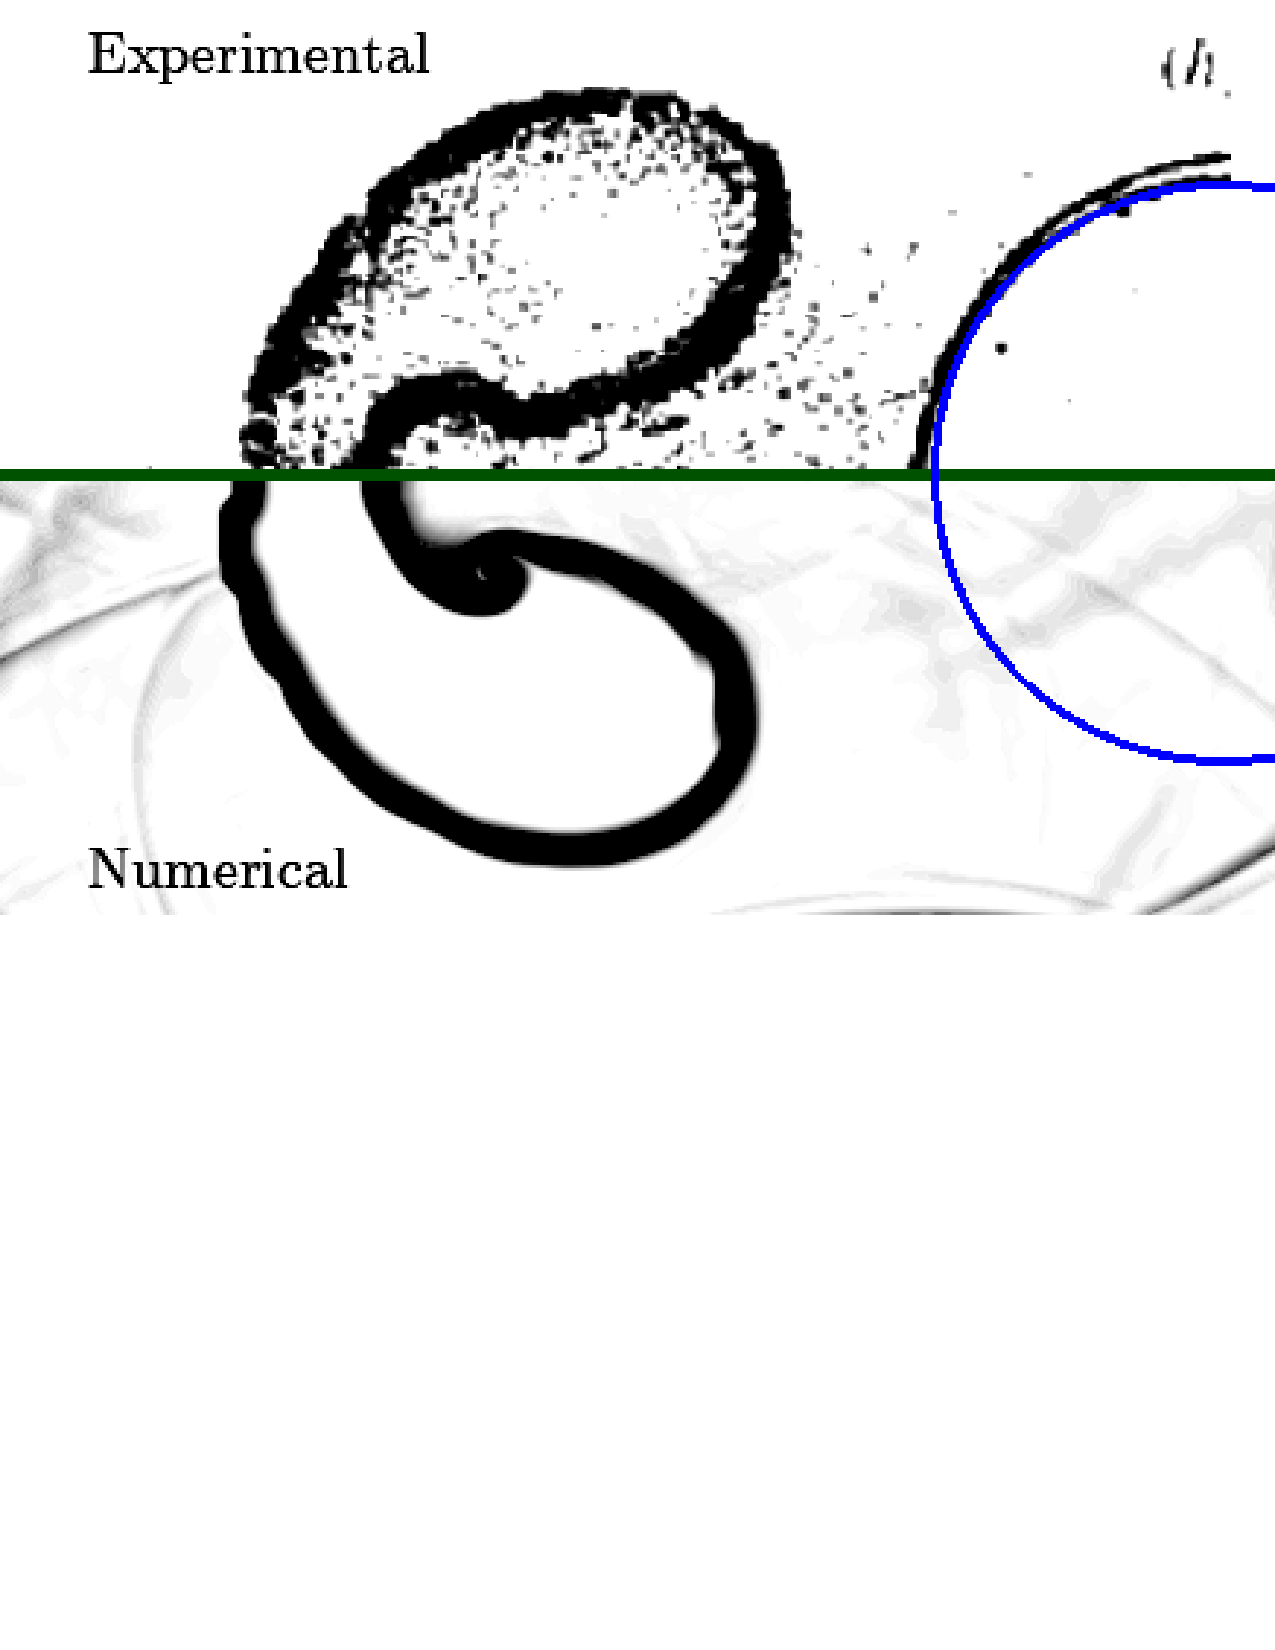
\includegraphics[width=0.3\linewidth]{results/helium_cropped.pdf} % Adjust the path and size
%	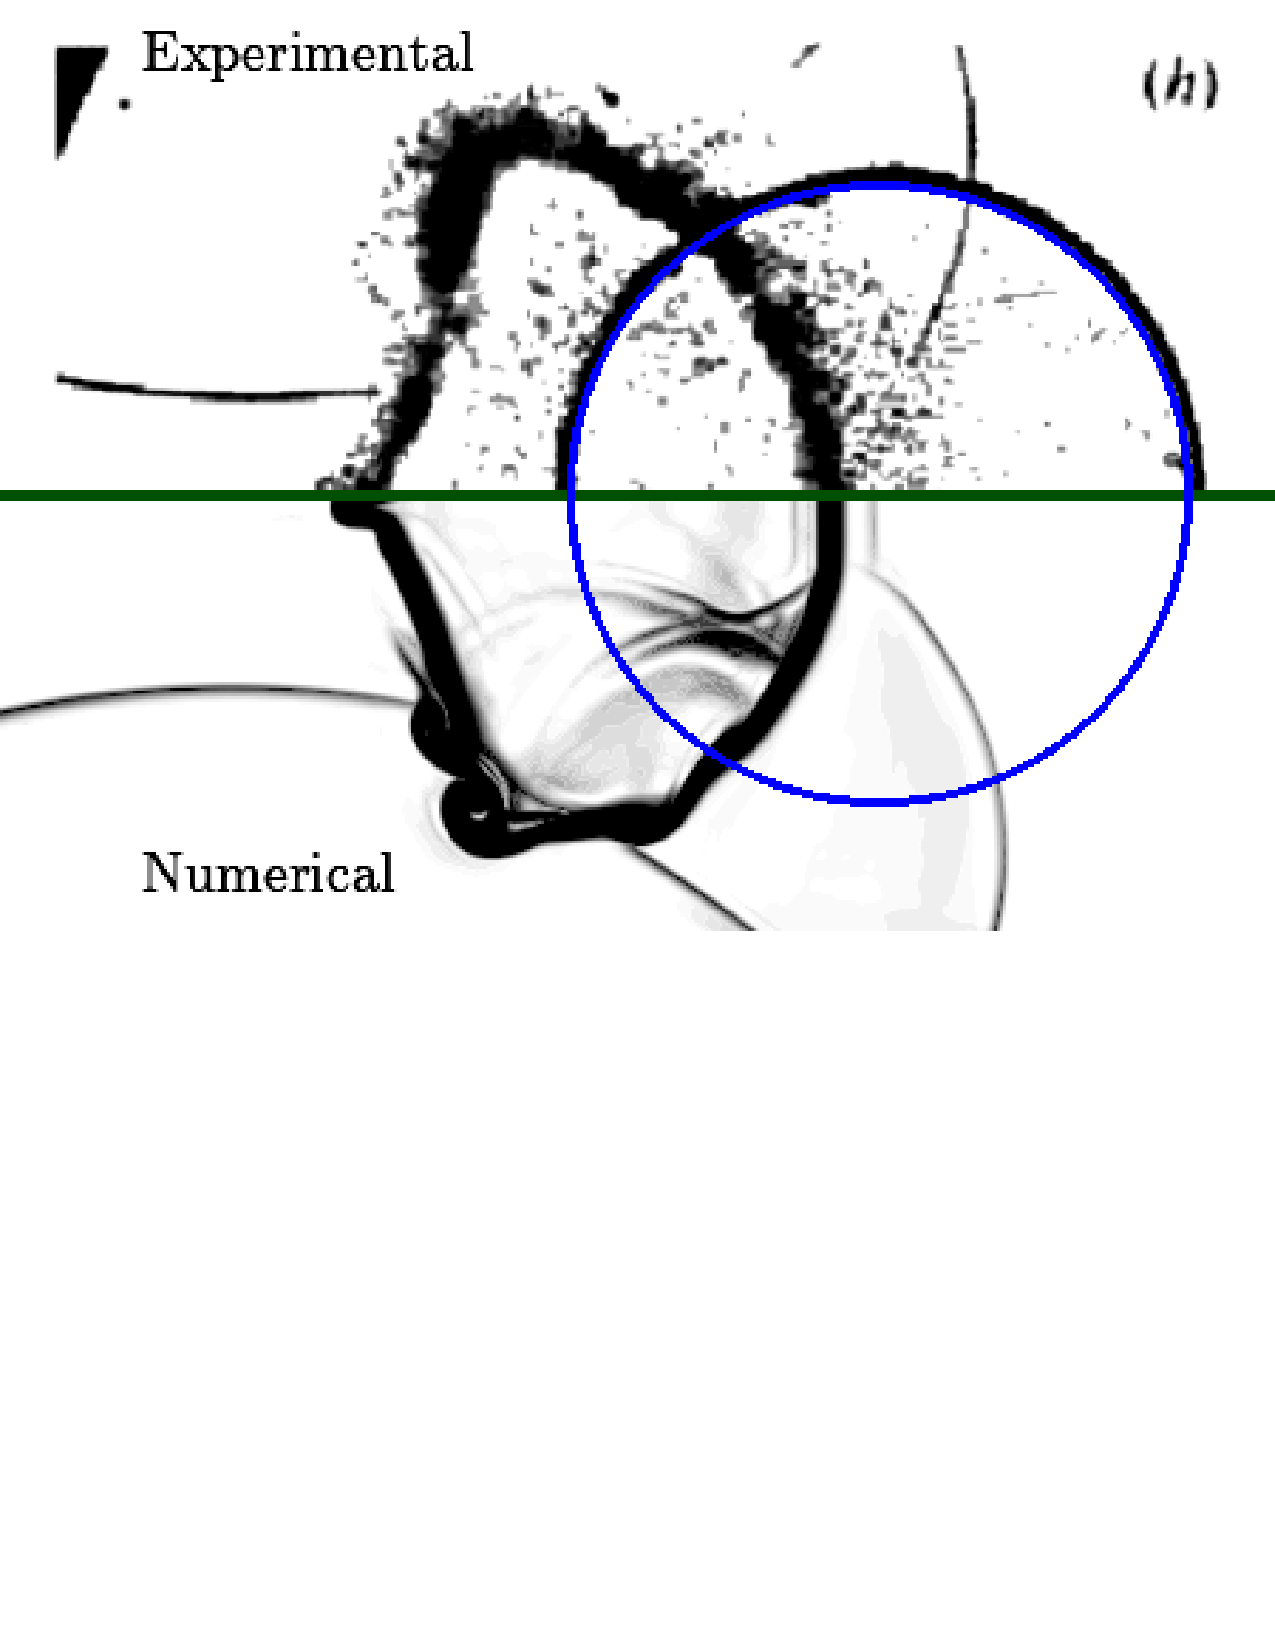
\includegraphics[width=0.3\linewidth]{results/r22_cropped.pdf} % Adjust the path and size



\end{frame}



\begin{frame}{Shock--Bubble Interaction}
	\centering
	\begin{minipage}[t]{0.72\textwidth}
		\centering
		\textbf{Helium} % Display the caption as bold text
		% First set of images
		\foreach \index in {1, ..., 31} {
			\only<\index>{ % Display only the current index
				\includegraphics[width=1.0\textwidth]{figure/simulation_frames_helium/frame_\index.png}
				\vspace{0.5em} % Add vertical space between images
				}
			}
			%Trick
			\only<32>{ % Display only the current index
				\includegraphics[width=1.0\textwidth]{figure/simulation_frames_helium/frame_31.png}
				\vspace{0.5em} % Add vertical space between images
			}
	\end{minipage}    
	\\ % Add horizontal space between minipages
	\begin{minipage}[t]{0.72\textwidth}
		\centering
		\textbf{R-22} % Display the caption as bold text
		% Second set of images
		\foreach \index in {1, ..., 31} {
			\only<\index>{ % Display only the current index
				\includegraphics[width=1.0\textwidth]{figure/simulation_frames_r22/frame_\index.png}
				\vspace{0.5em} % Add vertical space between images
				}
			}
			\only<32>{ % Display only the current index
				\includegraphics[width=1.0\textwidth]{figure/simulation_frames_r22/frame_31.png}
				\vspace{0.5em} % Add vertical space between images
			}
	\end{minipage}    
\end{frame}


\begin{frame}{Shock--Bubble Interaction\footnote{{\tiny J.-F. Haas, B. Sturtevant, 1987, Interaction of weak shock waves with cylindrical and spherical gas inhomogeneities.}}}
\centering

\begin{figure}[h]
	\centering
	\begin{subfigure}{0.45\linewidth}
		\centering
		\caption*{\textbf{Helium}}
		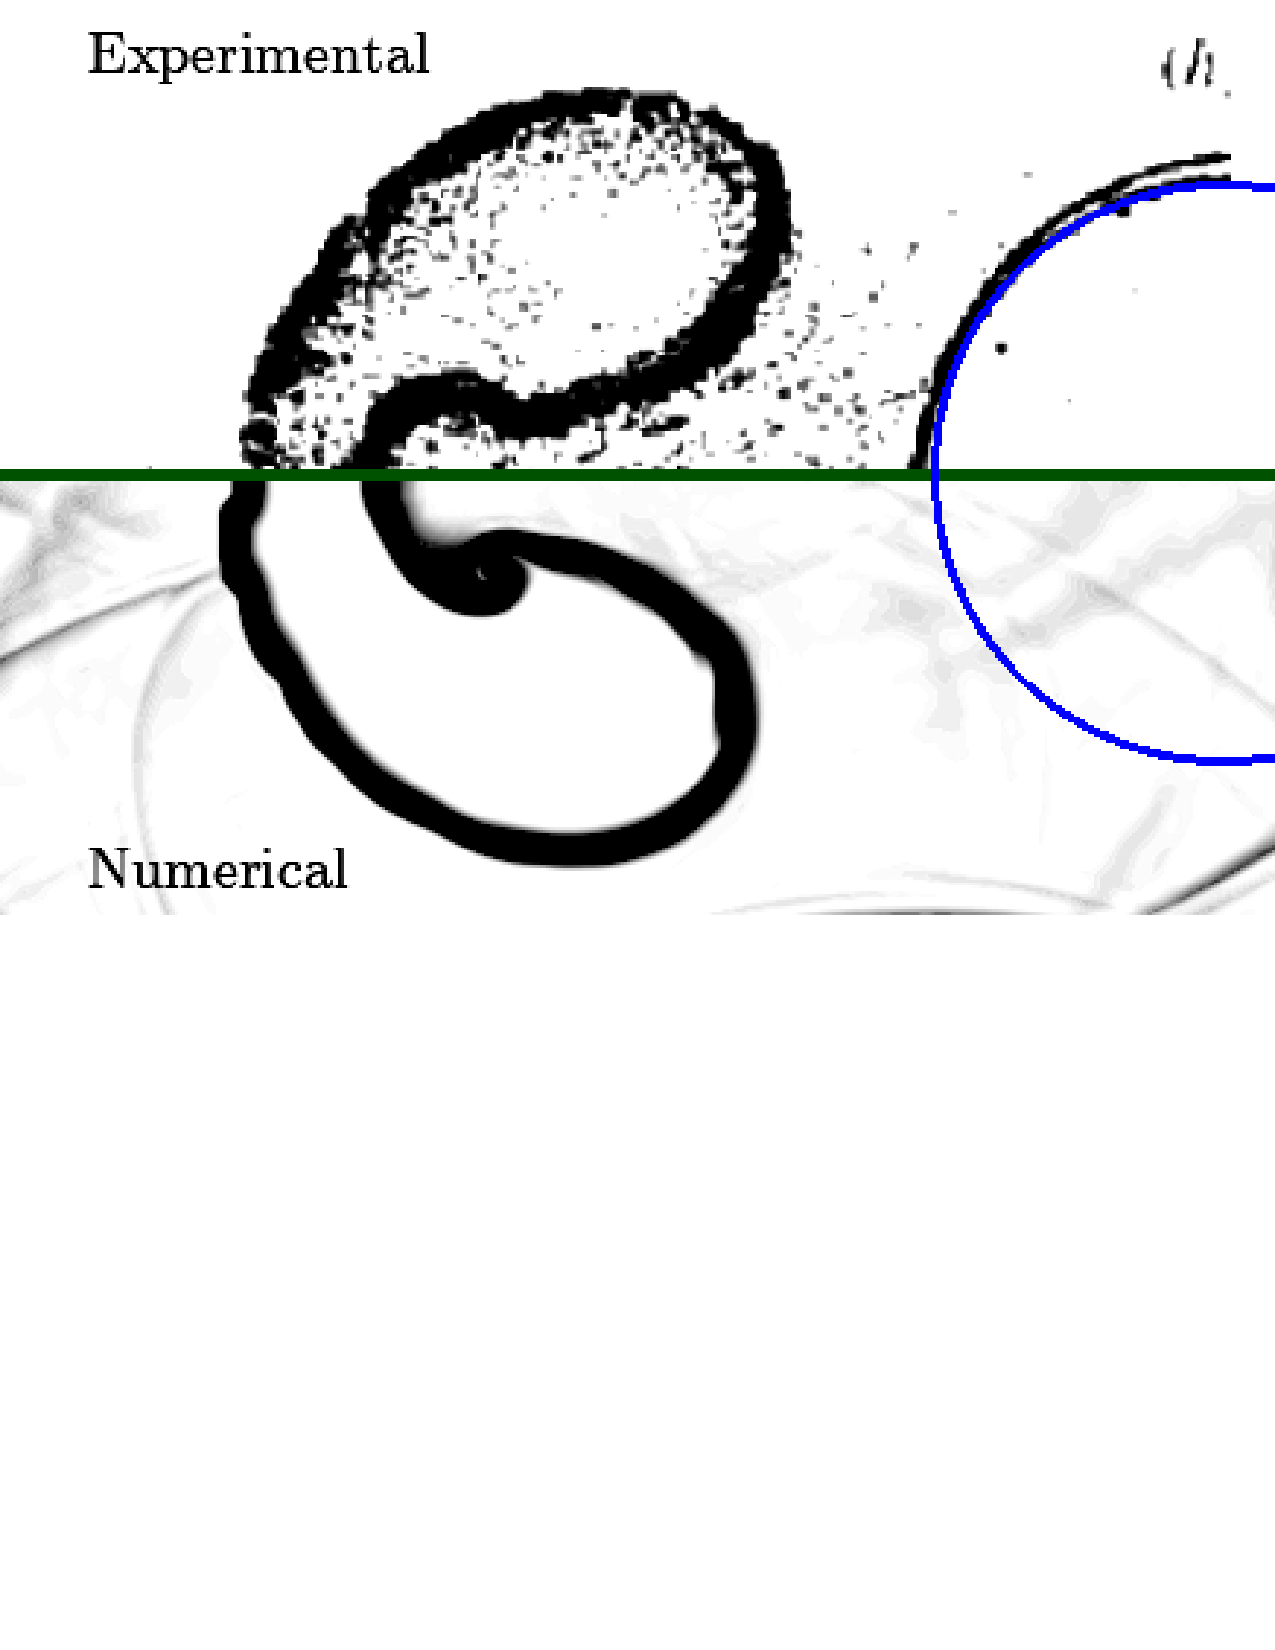
\includegraphics[width=\linewidth]{results/helium_cropped.pdf} % Adjust the path and size
	\end{subfigure}\hspace{1em} % Horizontal spacing
	\begin{subfigure}{0.45\linewidth}
		\centering
		\caption*{\textbf{R-22}}
		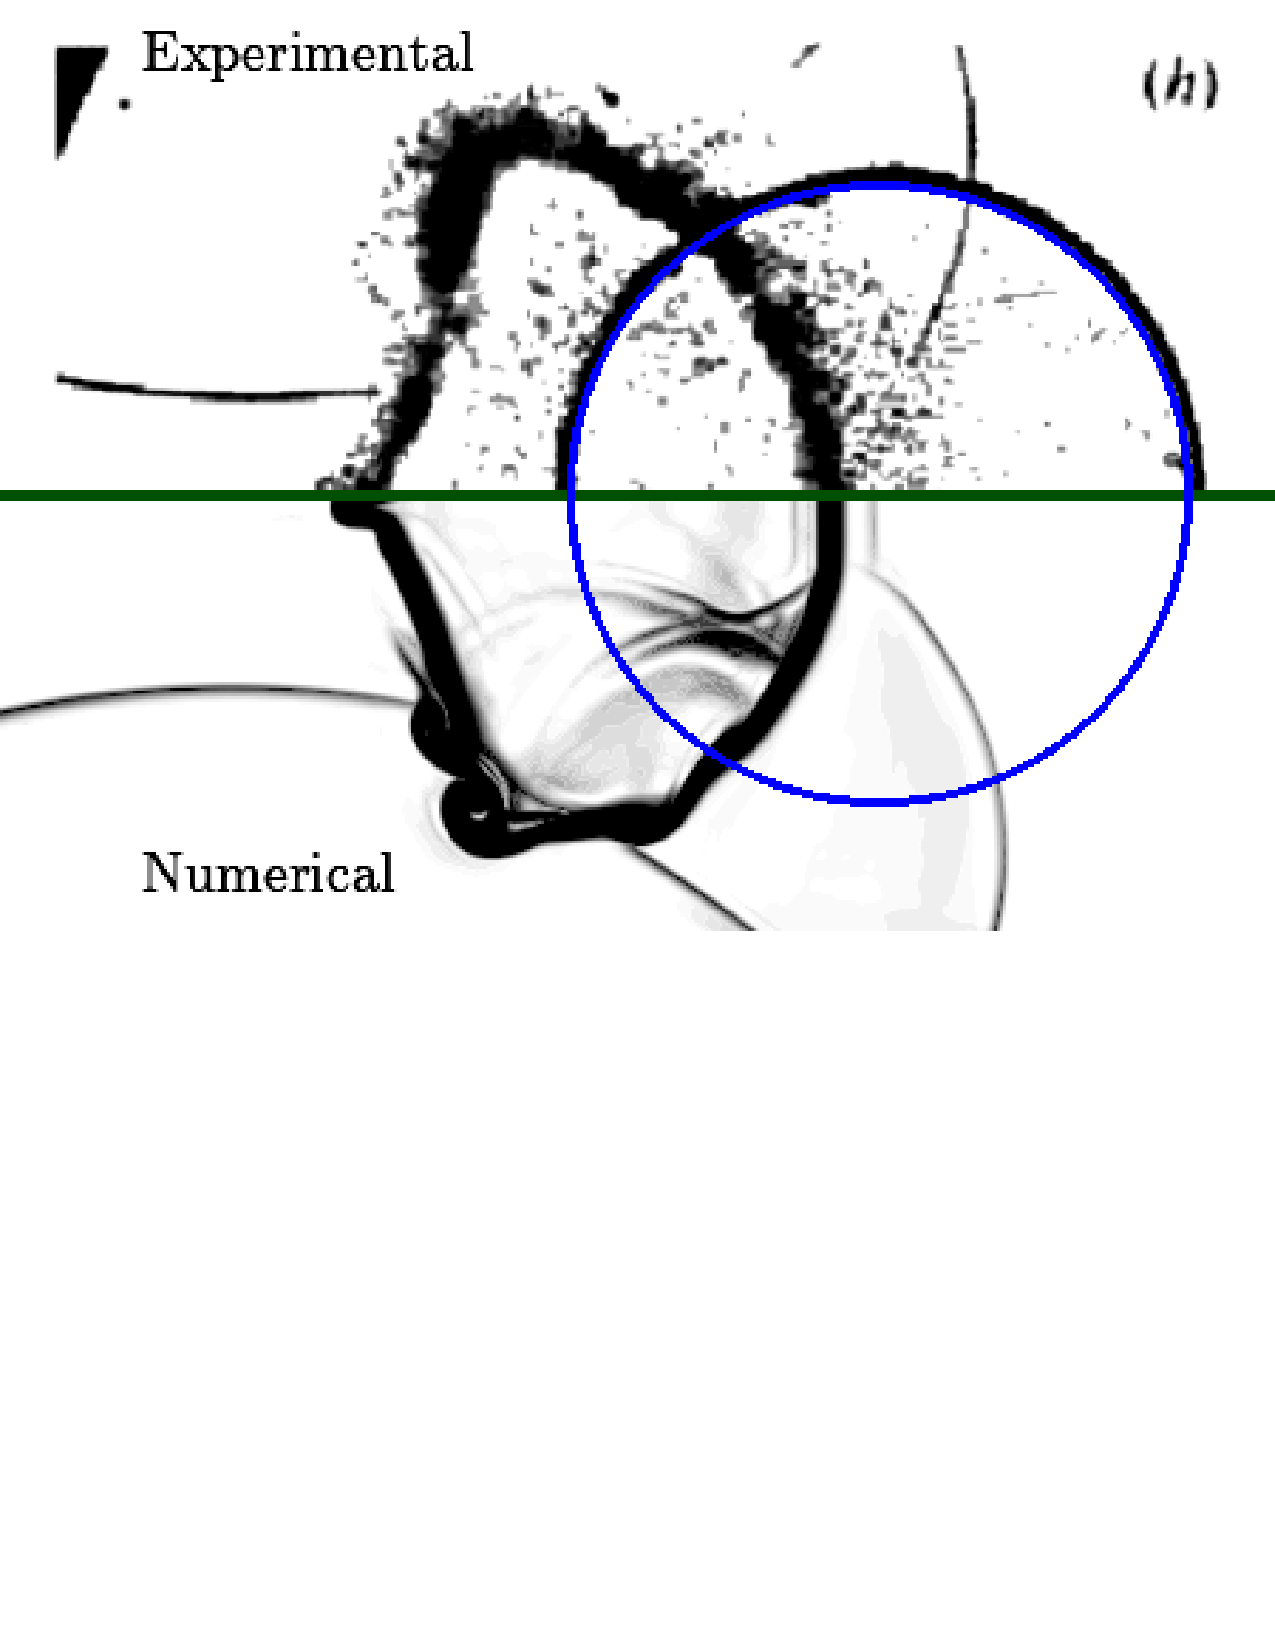
\includegraphics[width=\linewidth]{results/r22_cropped.pdf} % Adjust the path and size
	\end{subfigure}
\end{figure}

\vspace{-7em}

\end{frame}

\section{Conclusions}
\frame\sectionpage


\begin{frame}
	\frametitle{Conclusions}
	
\begin{itemize}
	\item Novel FV AF scheme with $\textcolor{blue}{\uvec{U}},\textcolor{red}{\uvec{V}}$ cell averages on staggered meshes 
	\begin{itemize}
		\item $\textcolor{blue}{\uvec{U}}$ updated with reconstructed values from $\textcolor{red}{\uvec{V}}$
		\item $\textcolor{red}{\uvec{V}}$ updated independently with \textcolor{violet}{PC} 
		\item Conservative post--processing
	\end{itemize}
	\item Application to multifluid with level set approach: $\textcolor{red}{(\rho \phi)}$ added to $\textcolor{red}{\uvec{V}}$
	
	
	
\end{itemize}
	
	
\end{frame}

\begin{frame}[label=THEEND]
\frametitle{The End}

\centering Thank you


{\tiny R. Abgrall, A. Chertock, A. Kurganov, L. Micalizzi, A New Semi-Discrete Finite-Volume Active Flux Method for Hyperbolic Conservation Laws, 2025}

\end{frame}

\section*{Backup slides}




\end{document}

